% Options for packages loaded elsewhere
\PassOptionsToPackage{unicode}{hyperref}
\PassOptionsToPackage{hyphens}{url}
%
\documentclass[
  man, donotrepeattitle,floatsintext]{apa6}
\usepackage{amsmath,amssymb}
\usepackage{iftex}
\ifPDFTeX
  \usepackage[T1]{fontenc}
  \usepackage[utf8]{inputenc}
  \usepackage{textcomp} % provide euro and other symbols
\else % if luatex or xetex
  \usepackage{unicode-math} % this also loads fontspec
  \defaultfontfeatures{Scale=MatchLowercase}
  \defaultfontfeatures[\rmfamily]{Ligatures=TeX,Scale=1}
\fi
\usepackage{lmodern}
\ifPDFTeX\else
  % xetex/luatex font selection
\fi
% Use upquote if available, for straight quotes in verbatim environments
\IfFileExists{upquote.sty}{\usepackage{upquote}}{}
\IfFileExists{microtype.sty}{% use microtype if available
  \usepackage[]{microtype}
  \UseMicrotypeSet[protrusion]{basicmath} % disable protrusion for tt fonts
}{}
\makeatletter
\@ifundefined{KOMAClassName}{% if non-KOMA class
  \IfFileExists{parskip.sty}{%
    \usepackage{parskip}
  }{% else
    \setlength{\parindent}{0pt}
    \setlength{\parskip}{6pt plus 2pt minus 1pt}}
}{% if KOMA class
  \KOMAoptions{parskip=half}}
\makeatother
\usepackage{xcolor}
\usepackage{graphicx}
\makeatletter
\def\maxwidth{\ifdim\Gin@nat@width>\linewidth\linewidth\else\Gin@nat@width\fi}
\def\maxheight{\ifdim\Gin@nat@height>\textheight\textheight\else\Gin@nat@height\fi}
\makeatother
% Scale images if necessary, so that they will not overflow the page
% margins by default, and it is still possible to overwrite the defaults
% using explicit options in \includegraphics[width, height, ...]{}
\setkeys{Gin}{width=\maxwidth,height=\maxheight,keepaspectratio}
% Set default figure placement to htbp
\makeatletter
\def\fps@figure{htbp}
\makeatother
\setlength{\emergencystretch}{3em} % prevent overfull lines
\providecommand{\tightlist}{%
  \setlength{\itemsep}{0pt}\setlength{\parskip}{0pt}}
\setcounter{secnumdepth}{-\maxdimen} % remove section numbering
% Make \paragraph and \subparagraph free-standing
\makeatletter
\ifx\paragraph\undefined\else
  \let\oldparagraph\paragraph
  \renewcommand{\paragraph}{
    \@ifstar
      \xxxParagraphStar
      \xxxParagraphNoStar
  }
  \newcommand{\xxxParagraphStar}[1]{\oldparagraph*{#1}\mbox{}}
  \newcommand{\xxxParagraphNoStar}[1]{\oldparagraph{#1}\mbox{}}
\fi
\ifx\subparagraph\undefined\else
  \let\oldsubparagraph\subparagraph
  \renewcommand{\subparagraph}{
    \@ifstar
      \xxxSubParagraphStar
      \xxxSubParagraphNoStar
  }
  \newcommand{\xxxSubParagraphStar}[1]{\oldsubparagraph*{#1}\mbox{}}
  \newcommand{\xxxSubParagraphNoStar}[1]{\oldsubparagraph{#1}\mbox{}}
\fi
\makeatother
% definitions for citeproc citations
\NewDocumentCommand\citeproctext{}{}
\NewDocumentCommand\citeproc{mm}{%
  \begingroup\def\citeproctext{#2}\cite{#1}\endgroup}
\makeatletter
 % allow citations to break across lines
 \let\@cite@ofmt\@firstofone
 % avoid brackets around text for \cite:
 \def\@biblabel#1{}
 \def\@cite#1#2{{#1\if@tempswa , #2\fi}}
\makeatother
\newlength{\cslhangindent}
\setlength{\cslhangindent}{1.5em}
\newlength{\csllabelwidth}
\setlength{\csllabelwidth}{3em}
\newenvironment{CSLReferences}[2] % #1 hanging-indent, #2 entry-spacing
 {\begin{list}{}{%
  \setlength{\itemindent}{0pt}
  \setlength{\leftmargin}{0pt}
  \setlength{\parsep}{0pt}
  % turn on hanging indent if param 1 is 1
  \ifodd #1
   \setlength{\leftmargin}{\cslhangindent}
   \setlength{\itemindent}{-1\cslhangindent}
  \fi
  % set entry spacing
  \setlength{\itemsep}{#2\baselineskip}}}
 {\end{list}}
\usepackage{calc}
\newcommand{\CSLBlock}[1]{\hfill\break\parbox[t]{\linewidth}{\strut\ignorespaces#1\strut}}
\newcommand{\CSLLeftMargin}[1]{\parbox[t]{\csllabelwidth}{\strut#1\strut}}
\newcommand{\CSLRightInline}[1]{\parbox[t]{\linewidth - \csllabelwidth}{\strut#1\strut}}
\newcommand{\CSLIndent}[1]{\hspace{\cslhangindent}#1}
\ifLuaTeX
\usepackage[bidi=basic]{babel}
\else
\usepackage[bidi=default]{babel}
\fi
\babelprovide[main,import]{english}
% get rid of language-specific shorthands (see #6817):
\let\LanguageShortHands\languageshorthands
\def\languageshorthands#1{}
% Manuscript styling
\usepackage{upgreek}
\captionsetup{font=singlespacing,justification=justified}

% Table formatting
\usepackage{longtable}
\usepackage{lscape}
% \usepackage[counterclockwise]{rotating}   % Landscape page setup for large tables
\usepackage{multirow}		% Table styling
\usepackage{tabularx}		% Control Column width
\usepackage[flushleft]{threeparttable}	% Allows for three part tables with a specified notes section
\usepackage{threeparttablex}            % Lets threeparttable work with longtable

% Create new environments so endfloat can handle them
% \newenvironment{ltable}
%   {\begin{landscape}\centering\begin{threeparttable}}
%   {\end{threeparttable}\end{landscape}}
\newenvironment{lltable}{\begin{landscape}\centering\begin{ThreePartTable}}{\end{ThreePartTable}\end{landscape}}

% Enables adjusting longtable caption width to table width
% Solution found at http://golatex.de/longtable-mit-caption-so-breit-wie-die-tabelle-t15767.html
\makeatletter
\newcommand\LastLTentrywidth{1em}
\newlength\longtablewidth
\setlength{\longtablewidth}{1in}
\newcommand{\getlongtablewidth}{\begingroup \ifcsname LT@\roman{LT@tables}\endcsname \global\longtablewidth=0pt \renewcommand{\LT@entry}[2]{\global\advance\longtablewidth by ##2\relax\gdef\LastLTentrywidth{##2}}\@nameuse{LT@\roman{LT@tables}} \fi \endgroup}

% \setlength{\parindent}{0.5in}
% \setlength{\parskip}{0pt plus 0pt minus 0pt}

% Overwrite redefinition of paragraph and subparagraph by the default LaTeX template
% See https://github.com/crsh/papaja/issues/292
\makeatletter
\renewcommand{\paragraph}{\@startsection{paragraph}{4}{\parindent}%
  {0\baselineskip \@plus 0.2ex \@minus 0.2ex}%
  {-1em}%
  {\normalfont\normalsize\bfseries\itshape\typesectitle}}

\renewcommand{\subparagraph}[1]{\@startsection{subparagraph}{5}{1em}%
  {0\baselineskip \@plus 0.2ex \@minus 0.2ex}%
  {-\z@\relax}%
  {\normalfont\normalsize\itshape\hspace{\parindent}{#1}\textit{\addperi}}{\relax}}
\makeatother

\makeatletter
\usepackage{etoolbox}
\patchcmd{\maketitle}
  {\section{\normalfont\normalsize\abstractname}}
  {\section*{\normalfont\normalsize\abstractname}}
  {}{\typeout{Failed to patch abstract.}}
\patchcmd{\maketitle}
  {\section{\protect\normalfont{\@title}}}
  {\section*{\protect\normalfont{\@title}}}
  {}{\typeout{Failed to patch title.}}
\makeatother

\usepackage{xpatch}
\makeatletter
\xapptocmd\appendix
  {\xapptocmd\section
    {\addcontentsline{toc}{section}{\appendixname\ifoneappendix\else~\theappendix\fi: #1}}
    {}{\InnerPatchFailed}%
  }
{}{\PatchFailed}
\makeatother
\usepackage{lineno}

\linenumbers
\usepackage{csquotes}
\usepackage{float} \floatplacement{figure}{H} \newcommand{\beginsupplement}{\setcounter{table}{0}  \renewcommand{\thetable}{S\arabic{table}} \setcounter{figure}{0} \renewcommand{\thefigure}{S\arabic{figure}}}
\ifLuaTeX
  \usepackage{selnolig}  % disable illegal ligatures
\fi
\usepackage{bookmark}
\IfFileExists{xurl.sty}{\usepackage{xurl}}{} % add URL line breaks if available
\urlstyle{same}
\hypersetup{
  pdftitle={ManyBabies2 Supplemental Material},
  pdflang={en-EN},
  hidelinks,
  pdfcreator={LaTeX via pandoc}}

\title{ManyBabies2 Supplemental Material}
\author{\phantom{0}}
\date{}


\shorttitle{Supplemental Material}

\affiliation{\phantom{0}}

\begin{document}
\maketitle

\setcounter{table}{0}  \renewcommand{\thetable}{S\arabic{table}} \setcounter{figure}{0} \renewcommand{\thefigure}{S\arabic{figure}}

This document contains supplemental material of the manuscript:

Schuwerk, T.*, Kampis, D.*, et al.~(2025, XXX XX). Action anticipation based on an agent's epistemic state in toddlers and adults. {[}Manuscript submitted for publication{]} (*shared co-first authorship).

\section{S1. Pilot Studies}\label{s1.-pilot-studies}

The familiarization trials were developed to convey information that is necessary for correct action predictions in this paradigm. First, the agent's goal is introduced, i.e.~the chaser wants to catch their partner (the chasee). Second, the situational constraints of the scene are shown. A barrier (fence) divides the scene so that the other side can only be reached by going through a y-shaped tunnel. Yet, it had to be clear that the fence is not a visual barrier, meaning that the chaser can see everything that takes place on the other side. Third, the familiarization trials should teach the timing of events, particularly, how much time the chaser spends in the tunnel and when their reappearance is to be expected. We piloted the stimuli with adults and toddlers between 18 and 27 months of age, the core age range of our main study. All analysis scripts can be found on GitHub (\url{https://github.com/manybabies/mb2-analysis}).

\subsection{Pilot 1}\label{pilot-1}

In the first pilot study, we wanted to get an estimate of the level of correct goal-based action predictions with these novel stimuli. We presented a total of eight familiarization trials. An observation of changes in the anticipation rate over trials would help us to determine the optimal number of familiarization trials. Further, we used this pilot to test the general procedure (i.e., data collection in different labs, preprocessing and analysis of raw gaze data from different eye-trackers). We also checked whether gaze patterns indicated any issues with perceptual properties of stimuli, such as distracting visual saliencies. Data for this pilot study was collected between February and July 2019.

\subsubsection{Methods}\label{methods}

\paragraph{Participants.}\label{participants.}

Seven labs\footnote{The contributing labs were: CEU Cog Dev Center, Central European University, Budapest; Babylab Copenhagen, University of Copenhagen, Denmark; Göttinger Kindsköpfe, Georg-August-Universität Göttingen, Germany; LMU Babylab, Ludwig-Maximilians-Universität München, Germany; Babylab Uni Trento, University of Trento, Italy; Center for Infant Cognition, University of British Columbia, Canada; Infant Learning and Development Lab, University of Chicago, USA} tested a total of 65 healthy full-term toddlers (28 males; Mean age = 23.14 months; range: 18.25 to 26.84 months). Data from eight additional toddlers were excluded from the analyses. Three did not complete the full experiment, another three did not complete at least six trials. Two toddlers had to be excluded due to technical problems with data collection (e.g., calibration of eye-tracker). At the trial level, four additional trials were excluded because the trial data was incomplete (as determined by not having at least 32 s of eye-tracking data for that trial, from the beginning to the end of the trial). A total of 42 adults were tested in three labs {[}5 males, 1 male/other, 1 N/C (not collected); Mean age = 24.10 years; range: 19 to 53 years{]}. One adult was excluded because this participant did not complete at least six trials. We asked contributing labs for a minimum sample size of 3-5 participants per age group. We reasoned that the resulting minimum total sample of 27-45 participants per age group would be large enough for an initial estimate of anticipatory looking (AL) behavior. The contributing labs were independently responsible for obtaining informed written consent and reimbursing participants. Each lab acquired ethics approval. Central data analyses only used de-identified data. Video recordings of participants were archived locally at each lab following the local data protection regulations.

\paragraph{Task and Procedure.}\label{task-and-procedure.}

Toddlers were tested in a quiet room of nurseries or laboratories, after their caregivers read and signed the informed consent form. They sat on an educator/caregiver's lap or on a car seat, centered in front of the monitor used to display the stimuli at a distance of about 60-80 cm. Educators or caregivers were instructed to remain silent and to wear black glasses or close their eyes to avoid erroneous tracking of their eyes. The experimenter was behind a curtain/room divider and controlled stimulus presentation. Depending on the lab setup, the following eye-tracking systems were used: Tobii T60 (two labs), Tobii T120 (two labs), EyeLink 1000 Plus (two labs), SMI250Redmobile (two labs), SMI iView X Hi-Speed 1250 (one lab). For each lab the following information was collected: type of eye-tracker apparatus, trial order condition (A or B), any procedural or technical error that occurred during the experimental session, location of the lab they were tested in (laboratory or nursery).
The task consisted of a calibration check, eight familiarization trials and another final calibration check. After an initial attention getter, participants were presented with the calibration check that consisted of an animated star with sound, moving and stopping at four locations. The familiarization trials were as described in the Methods section of the main study, with the following deviations: In the upper part of the tunnel there was a small window that allowed participants to watch the agents moving inside the upper part of the tunnel before it forked. Further, unlike in the final familiarization trial version, a chime sounded at the moment the chaser disappeared from the tunnel window, indicating the start of the anticipatory period. The starting location of the chasee (left or right half of the upper part of the scene) and the box the chasee ended up (left or right box) were counterbalanced, resulting in a total of four familiarization trial versions {[}started from the right and ended up in right box (RR); started from the right and ended up in left box (RL); started from the left and ended up in right box (LR); started from the left and ended up in left box (LL){]}. Each of these versions was presented twice in two pseudo-randomized orders (Order A: LL1, LR2, RR2, RR1, LL2, RL2, LR1, RL1; Order B: RL1 LR1, RL2, LL2, RR1, RR2, LR2, LL1). Half of the participants in each lab group were randomly assigned to one of the two orders.

\paragraph{Data Analysis.}\label{data-analysis.}

The labs exported the raw gaze data in the format the respective eye-tracking software allowed. The participants' demographic information and details about the test session were collected in standardized spreadsheets. Each lab provided the raw gaze data and de-identified demographic information with Google Drive. Data preprocessing was identical to the procedure of the current study. For details refer to the Methods section of the main manuscript.

\subsubsection{Results}\label{results}

\paragraph{Descriptive Statistics.}\label{descriptive-statistics.}

In Figure S1, we show the toddlers' proportion of first looks and the proportion looking at each of the critical AOIs (target, distractor, other) during the anticipatory period of each trial. Figure S2 (plots labeled pilot 1) shows the proportion of looking of toddlers and adults as a smooth curve, generated by binning the data and averaging the proportion looking at each time point across all participants. We saw robust evidence for looks to the target relative to the distractor during the anticipation period, as evidenced by the red lines being consistently higher than the blue lines. In Figure S2, we separated trials into two blocks (Trials 1-4 and Trials 5-8). For toddlers in Pilot 1, we see similar rates of anticipation for Trials 1-4, as in Trials 5-8. In fact, anticipation is slightly lower in Trials 5-8 than in Trials 1-4. For adults, we see an increase in the anticipation rate in Trials 5-8.
The heatmaps in Figure S3 illustrate the distribution of looks to scene locations during the anticipatory period. We found that a large proportion of anticipatory looks was directed to the tunnel exits. Substantially fewer looks fell onto the boxes. Unexpectedly, many looks were attracted by the tunnel window (the location where the chaser was last seen).

\begin{figure}

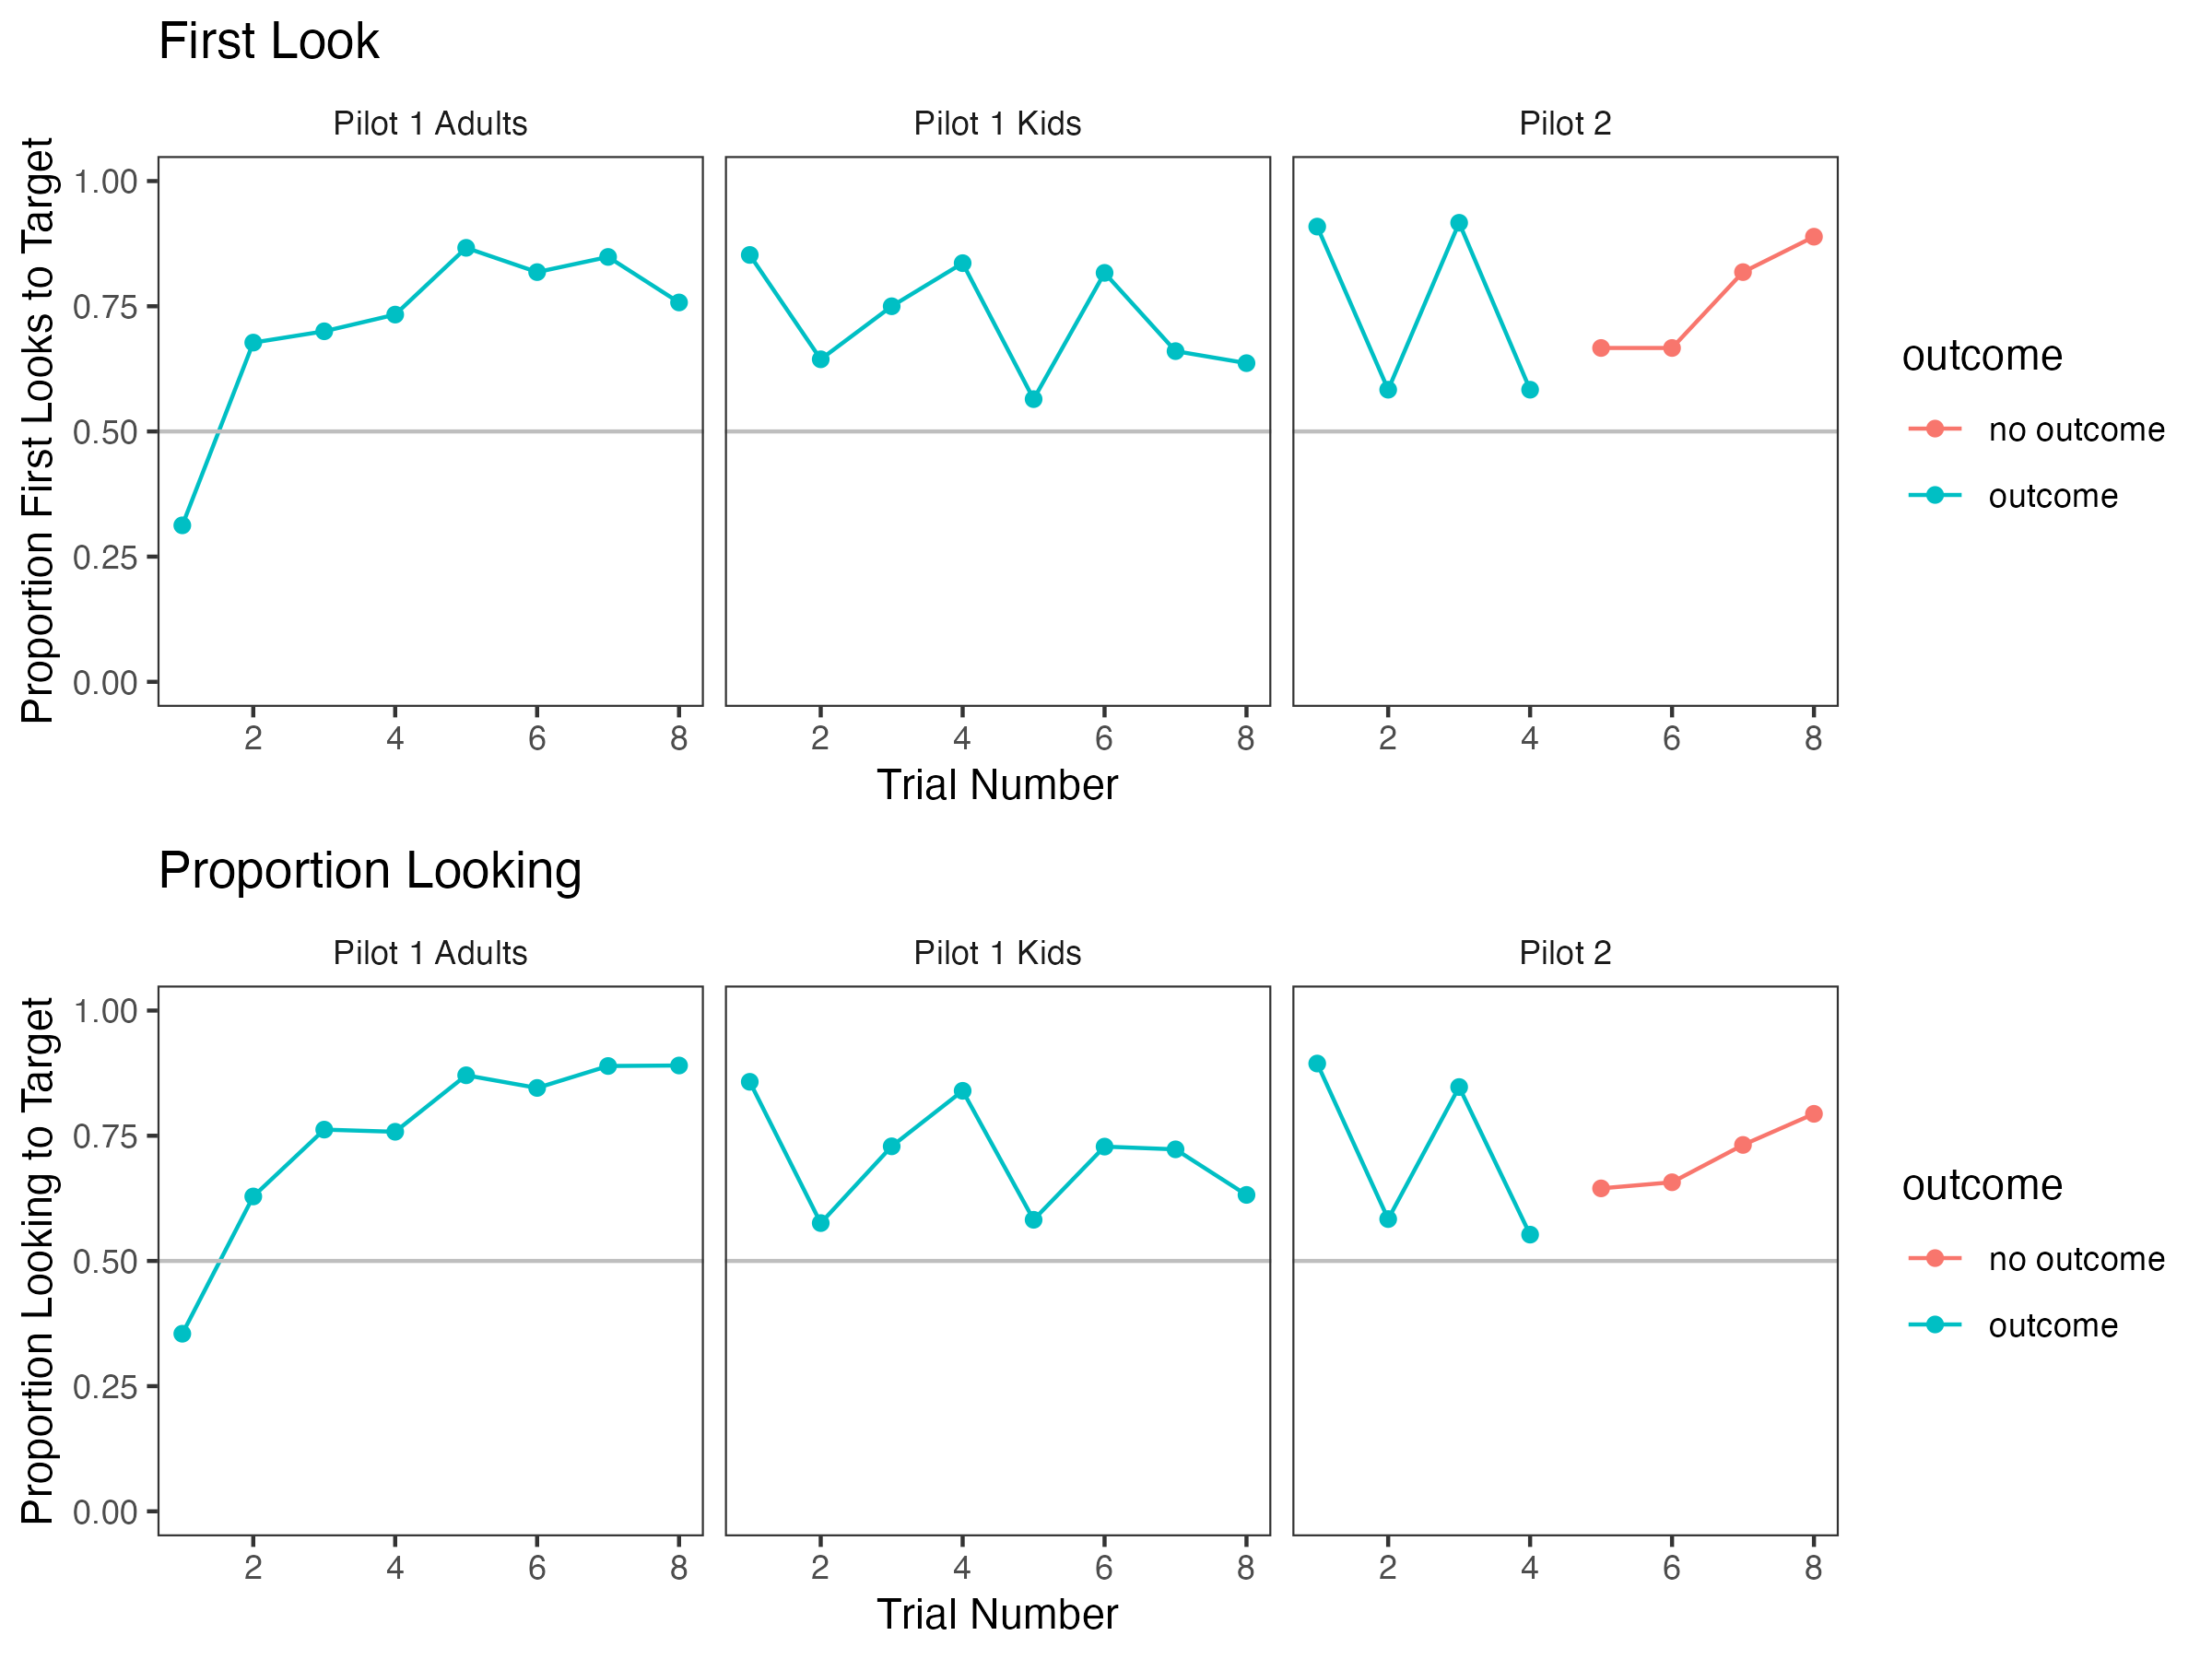
\includegraphics[width=6in]{/Users/mellischreiner/Documents/GitHub/mb2-analysis/paper/FigureS1} \hfill{}

\caption{First looks and proportion looking of children from Pilot 1 for each trial. \newline{} \textit{Note}. Top: proportion of first looks to the target as a function of trial number; Bottom: proportion looking score as a function of trial number.}\label{fig:figS1}
\end{figure}

\begin{figure}

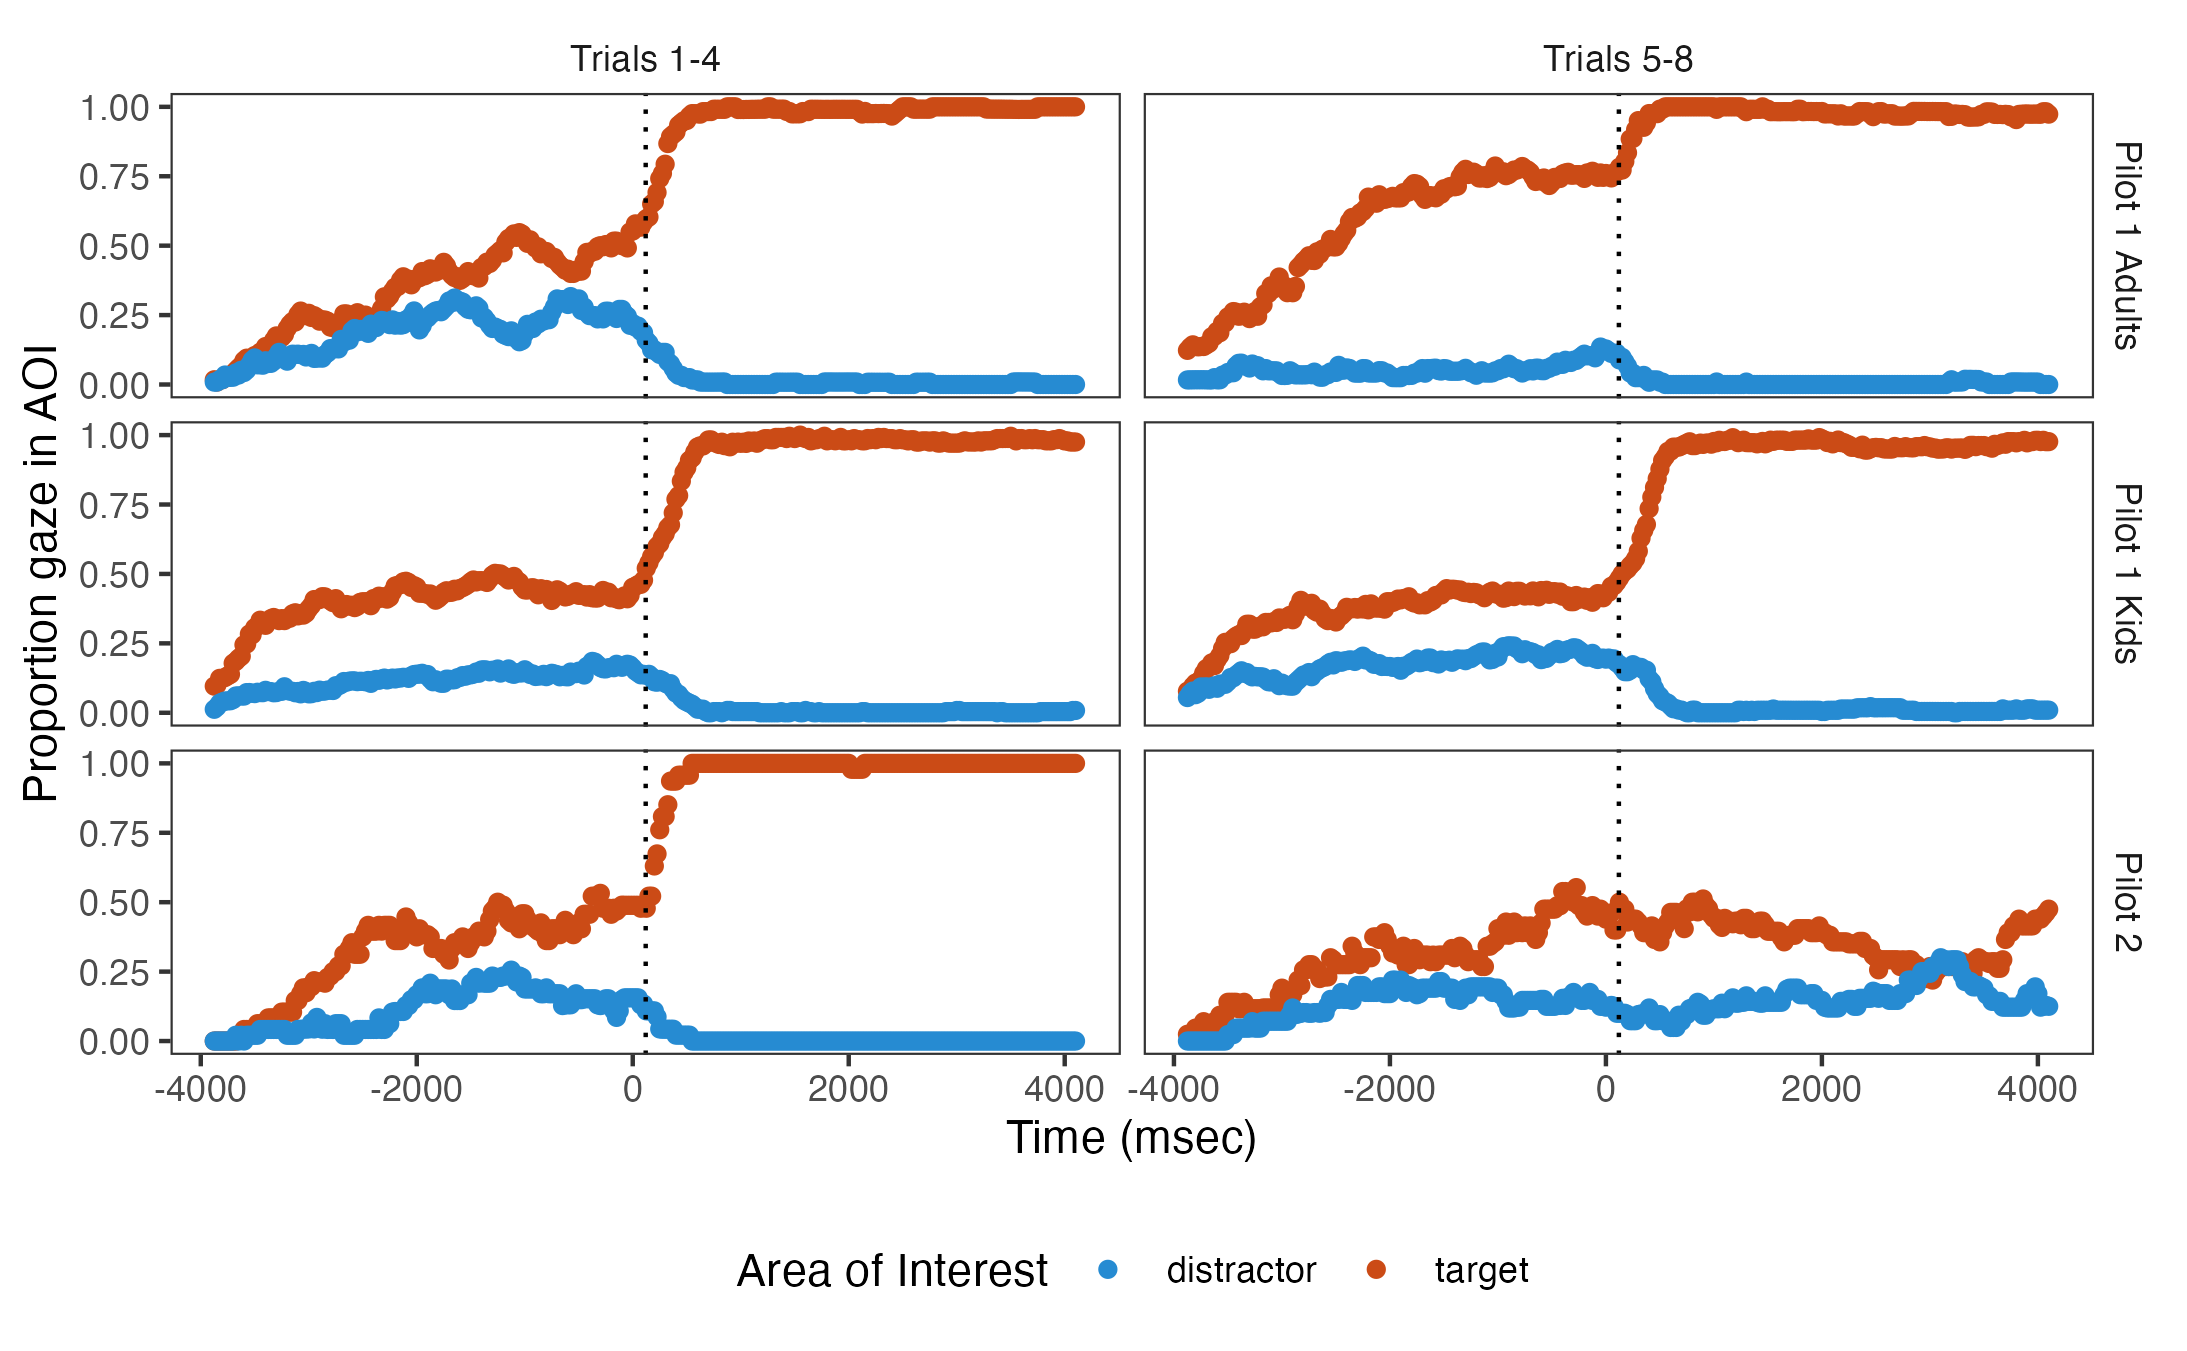
\includegraphics[width=6in]{/Users/mellischreiner/Documents/GitHub/mb2-analysis/paper/FigureS2} \hfill{}

\caption{Binned proportion looking, averaged across all participants and trials. \newline{} \textit{Note}. The left column comes from Trials 1-4, the right column from Trials 5-8. The vertical dotted line represents the disambiguation time. The red points represent looks to the target, the blue points represent looks to the distractor.}\label{fig:figS2}
\end{figure}

\begin{figure}

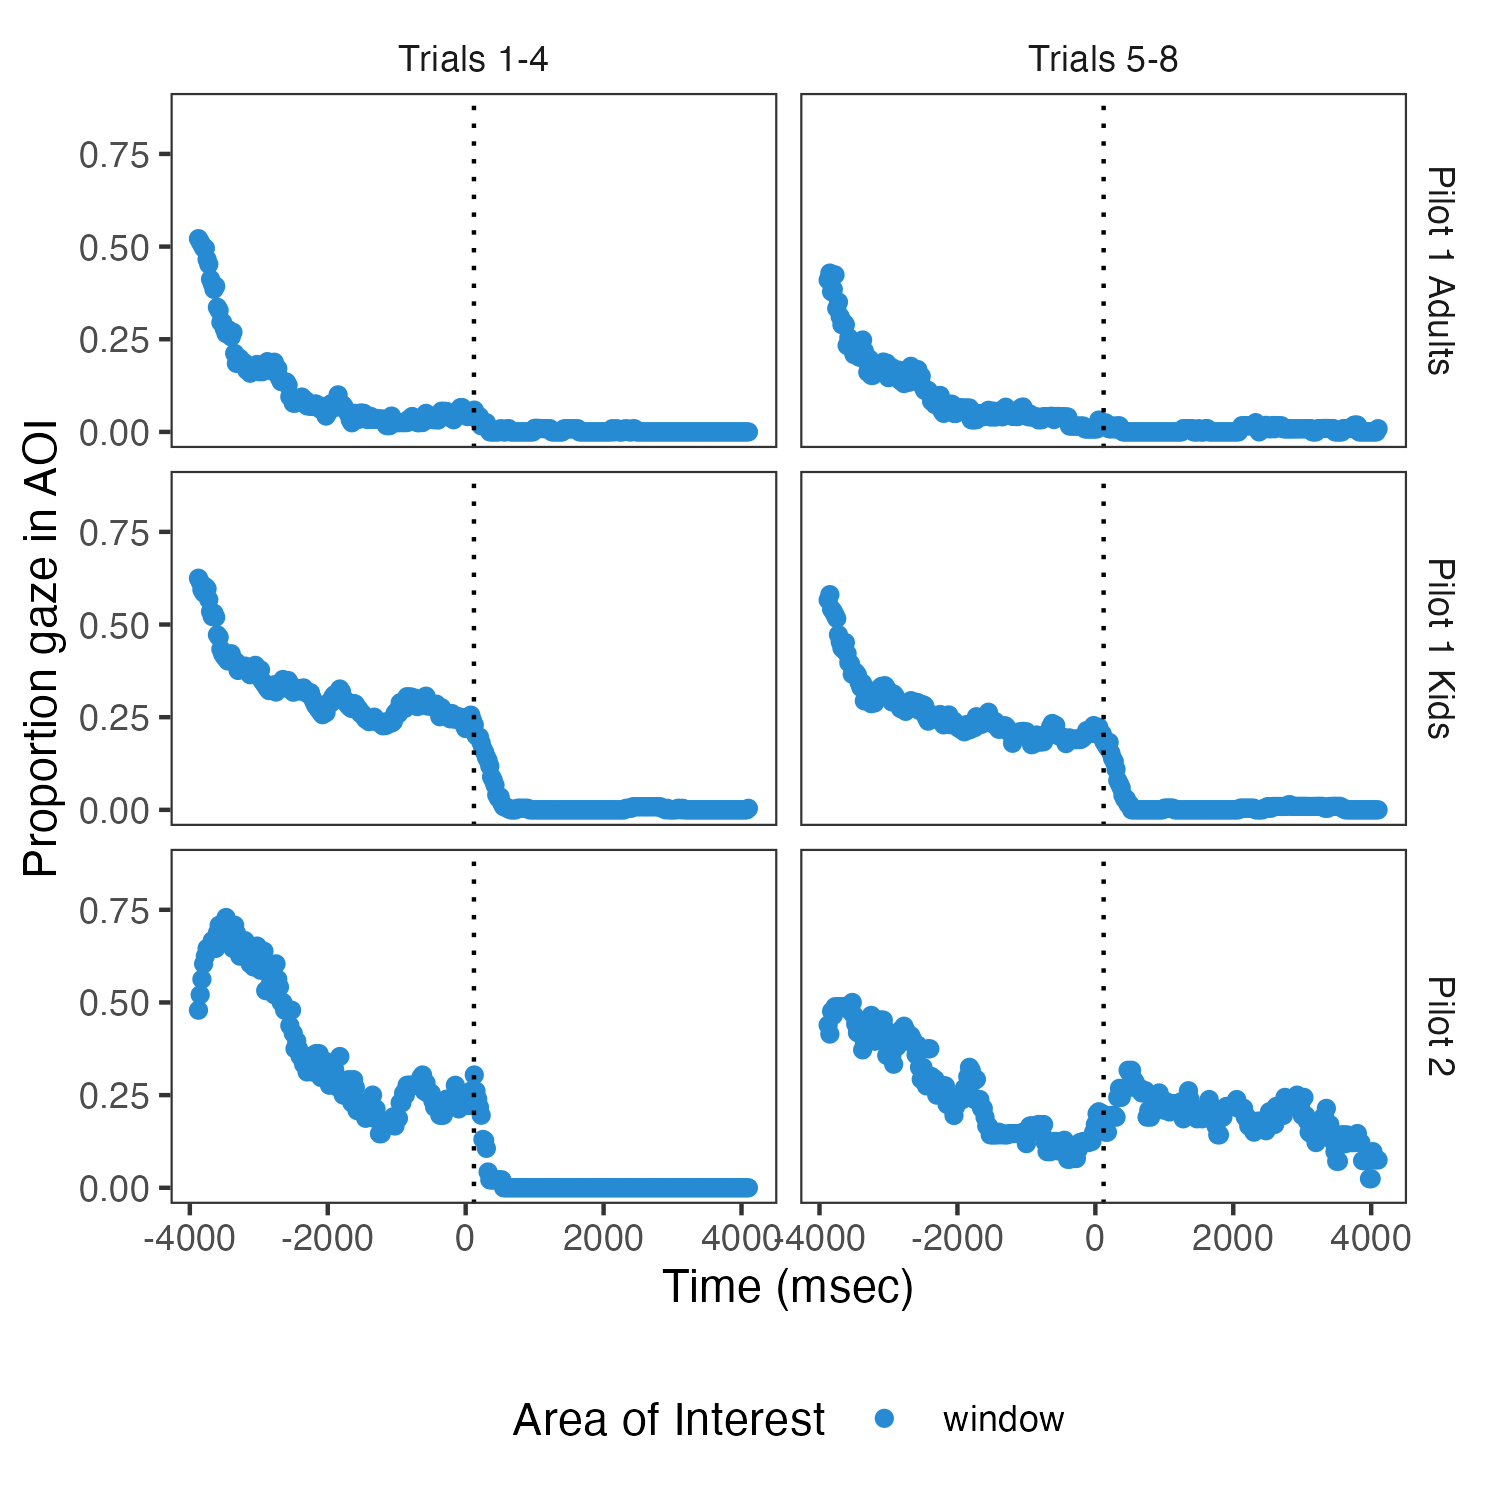
\includegraphics[width=6in]{/Users/mellischreiner/Documents/GitHub/mb2-analysis/paper/FigureS3} \hfill{}

\caption{Heatmaps showing the distribution of looks in the anticipatory period in Pilot Study 1 (left: adults; right: toddlers). \newline{} \textit{Note}. Larger and reddisher areas indicate a greater amount of looks toward the respective location.}\label{fig:figS3}
\end{figure}

\paragraph{Inferential statistics.}\label{inferential-statistics.}

To further assess the pilot data and test our proposed analysis described in the main text, we ran two Bayesian mixed effect models as described in the main manuscript, the first using first look location as the dependent variable and the second using proportional looking score as the dependent variable. For the first look analysis, we defined the first look location as in the main text (corresponding roughly to the first look of 150 ms or more in the same AOI). We calculated the proportion looking (\emph{p}) to the correct AOI during the full 4000 ms anticipatory window by correct AOI looks / (correct AOI looks + incorrect AOI looks), excluding looks outside of either AOI. The anticipatory eye movement window was defined 120 ms after the first frame when the chaser had completely entered the tunnel and 120 ms after the chaser reappeared from the tunnel.\\
Because we wanted to ask if participants were attentive and could still make predictive looks at the end of the familiarization phase, we coded the trial number such that the last trial during the familiarization phase (the 8th in pilot 1) is set to 0, with trials 1 through 7 are coded as -7 to -1, respectively. We used the priors described in the main text of our analysis plan. Our base model was as follows, where measure refers to the dependent variable (either first look or the proportional looking score):\\
\(Measure ~ 1 + trial\_number + (trial\_number | lab) + (trial\_number | participant).\)
We fitted a reduced model for model comparison:
\(Measure  ~ 0 + trial\_number + ( trial\_number | lab) + (trial\_number | participant).\)
We then calculated the Bayes factor, which we interpret as described in the main text.

\subparagraph{Toddlers.}\label{toddlers.}

For the first look analysis, the intercept estimate was .44, (CrI95\% = 0.07, 0.80). This corresponds to a point estimate of a 61\% probability of the first look to be mapped onto the target as opposed to the distractor. The Bayes factor comparing the model with and without the intercept was 1.52, which is inconclusive by our criteria (Schönbrodt \& Wagenmakers, 2018). For the proportional looking score main model, the model estimate for the intercept was 0.16 (CrI95\% = 0.10, 0.23). This can be interpreted as a point estimate of a 66\% probability of looking at the target. The Bayes factor was 493.25, which was strong evidence in favor of the full model and which strongly suggests that toddlers looked more towards the target than towards the distractor during the anticipation period.

\subparagraph{Adults.}\label{adults.}

For the first look analysis, we obtained a model estimate of 1.95 (CrI95\% = 1.42, 2.48). This corresponds to a probability of 88\% that the first look is to the target. The Bayes factor was \textgreater{} 1000, which was evidence in favor of the full model. For the Proportion Differential looking score analysis\footnote{We note that the base model for the Proportion Differential looking score analysis in adults had divergent issues. These issues were not resolved after adjusting the alpha level to a very high number (e.g., 0.999999). Thus, the results needed to be interpreted with caveat.}, the Bayes factor was also \textgreater{} 1000, which was evidence in favor of the full model. This suggested that adults had a higher proportion of looking at the target than chance level. The model estimate for the intercept was 0.46 (CrI95\% = 0.38, 0.54). Based on these analyses, it is clear that adults looked more to the target than the toddlers did, and it appears this was driven by Trials 5-8, as can be seen in Figure S2. Adults learn to anticipate the target and, on later trials, very rarely look at the distractor.

\subsubsection{Discussion}\label{discussion}

Based on the first pilot, we drew the following conclusions: (1) Toddlers and adults show anticipation during the anticipatory period, and thus the paradigm seems successful at eliciting anticipation. (2) Over the course of eight trials, toddlers and adults remained attentive and showed anticipatory behavior even during the last trial of the familiarization phase. (3) Four familiarization trials seem to be sufficient and there do not appear to be strong additional benefits of running additional trials. Crucially, trials five to eight did not help to increase the overall anticipation rate for toddlers, as shown in Figure S2. Note that in the adults sample AL slightly increased after trial 4. We nonetheless decided to use four familiarization trials in the main study because we reasoned that it is more important to avoid fatigue or boredom in the toddlers sample than to get even higher anticipation rates for adults.
It is important to note that our decision to include 4 familiarization trials is based on (1) conceptual and practical methodological considerations also considering previous studies and (2) the pilot study results. Replication studies of Southgate, Senju, and Csibra (2007) pointed to issues with the familiarization phase and that the two trials of the original study might not be enough to familiarize toddlers with the scenario (e.g., Kampis \& Southgate, 2020; Schuwerk, Priewasser, Sodian, \& Perner, 2018). On the other hand, to avoid unnecessarily increasing the overall length of the task and to prevent poor anticipatory looking due to fatigue or boredom, we did not want to include too many familiarization trials. In the discussions preceding the pilot data analysis, we came to the conclusion that four trials reflect such an optimal trade-off. The pilot data results of the toddlers then supported this decision insofar as we observed a looking bias towards the correct location already in trials 1-4, without additional benefit of trials 5-8. Due to the exploratory nature of the pilot studies, we refrained from running inferential statistics in addition to the visual inspection of the first look and proportion looking data, as well as of the time series illustration, which all converged on this interpretation (see supplementary Figure S1 and S2).
The duration of the anticipatory period was set based on durations used in previous studies. Earlier studies found action outcome-contingent anticipatory looking with anticipatory phases ranging between approximately 2-3.5 seconds (Low \& Watts, 2013; Meristo et al., 2012; Surian \& Geraci, 2012; Thoermer et al., 2012). To make sure we are not losing anticipatory looks by cutting off too early, we decided to use a time period of 4 seconds. The pilot data showed no evidence for a decline in anticipatory looking towards the end of the anticipatory period (see time series plot in S2), which supported this decision.
Further, the distribution of looks in the anticipatory period helped us to evaluate the appropriateness of our AOI dimension, in particular whether restricting AOIs to the tunnel exits not including the adjacent box optimally captures goal-directed anticipatory looks. By increasing the AOI dimensions so that they cover both the tunnel exit and the box, we could potentially detect more goal-directed anticipatory looks. On the other hand, looks to the box cannot unambiguously be interpreted as anticipations of the chaser's upcoming action. Participants might look to the box simply because this is where the chasee is, anticipating that the chasee might jump out of the box again. Thus, we concluded that restricting our AOIs to the tunnel exits --the location where the chaser will reappear-- is the more conservative and more unambiguously interpretable measure of goal-directed action prediction. The result of our pilot study corroborated this strategy. The larger proportion of anticipatory looks was indeed directed to the tunnel exits and not to the boxes. Based on this finding, we concluded that using the tunnel exit AOIs is the sharper measure of goal-directed action predictions without a substantial loss of looks that could also reflect action predictions but are directed elsewhere (e.g., to the box).
An unexpected result of Pilot 1 was that during the anticipatory period, many fixations were attracted by the tunnel window where the agent was last seen. This was potentially problematic since looking at the window could lead to a reduced amount of anticipatory looks to the target/distractor AOIs. Initially, the window was added to the tunnel with the aim to increase AL (cf., Surian \& Franchin, 2020). But the results suggested that it may have been distracting, and so we removed the window for Pilot 2.

\subsection{Pilot 2}\label{pilot-2}

To further hone our stimulus design, we conducted a second pilot. First, we removed the potentially distracting tunnel window from all trials in Pilot 2. Second, we tested another method to increase AL. We asked whether a chime as an arbitrary timing cue helps to elicit AL to the tunnel exits in (future) test trials in which the agent does not reappear at one of the tunnel exits (because these test trials stop after the end of the anticipatory phase without showing the agent's action outcome). To this end, we presented the first four familiarization trials showing the outcome associated with the chime, i.e., the chime announced the reappearance of the chaser, and four subsequent familiarization trials without an outcome, i.e., the chime sounded, but the chaser did not reappear. We reasoned that if participants learn in the first four trials that the chime indicates the chaser's reappearance, we should see an increase in AL right after the chime sounded. Further, this increase should also be observable in the last four trials in which the chaser does not reappear. Data collection for this pilot started in January 2020 and had to stop due to Covid-19 outbreak in March 2020.

\subsubsection{Methods}\label{methods-1}

\paragraph{Participants.}\label{participants.-1}

A total of 12 healthy full-term toddlers participated in the second pilot study (6 males; Mean age = 24.15 months; range: 19.14 months to 26.05 months). One additional toddler was tested but excluded from the analyses because this toddler did not complete at least six trials. An additional one trial was excluded as the toddler did not look at least 32 seconds during this trial. We asked five labs to contribute a minimal sample size of four toddlers. Yet, data collection had to stop due to the Covid-19 outbreak.

\paragraph{Task and Procedure.}\label{task-and-procedure.-1}

The task and procedure were similar to Pilot 1. In this study, the following eye-tracking systems were used: Tobii T60 (one lab), Tobii T120 (one lab), EyeLink 1000 Plus (two labs), and Tobii Pro Spectrum (one lab). After the initial attention getter, participants were presented with the calibration check as in Pilot 1, eight familiarization trials and at the end, again the calibration check. The familiarization trials started by showing the same scene as in pilot 1, except that the window was removed from the tunnel. The trials differed in whether they displayed an outcome (i.e., the chaser exits the tunnel and the two agents rejoin) or not (i.e., trial stopped after the anticipatory period). The first four trials showed the outcome, the last four trials did not. Unlike in the first pilot, the chime now sounded the moment the chaser reappeared at one of the tunnel exits in the outcome trials. In the no outcome trials, the chime sounded the same moment, yet now the chaser did not appear. Again, the trials were presented in two pseudo-randomized orders {[}Order A: outcome (LR, LL, RR, RL), no outcome (LL, RL, LR, RR); Order B: outcome (RL, RR, LL, LR), no outcome (RR, LR, RL, LL{]}. Half of the participants in each lab group were randomly assigned to one of two orders.

\paragraph{Data Analysis.}\label{data-analysis.-1}

Data preprocessing was analogous to Pilot 1.

\subsubsection{Results and Discussion}\label{results-and-discussion}

As can be seen in Figures S1 and S2, we found a similar pattern of results in both conditions of Pilot 2 (with outcome and without come) as we did in Pilot 1. We saw more looks directed towards the target than to the distractor. As described above, all trials in Pilot 2 lacked the tunnel window, whereas all trials in Pilot 1 included the tunnel window. Thus, we can assess the effect of the tunnel window by comparing Pilot 2 to Pilot 1. We found that the removal of the tunnel window did not appear to increase or decrease AL in Pilot 2 in any clear way. In fact, even after the removal of the window, a substantial amount of gaze was attracted towards the location where the window had been in Pilot 1 (for an illustration, see Figure S4). An explanation for this pattern of results is that not the window itself but its location in the center of the scene attracted visual attention. Previous research documented a central fixation bias in infants, toddlers and adults when viewing complex visual scenes (Tatler, 2007; van Renswoude et al., 2019).
By comparing the outcome and no outcome conditions in Pilot 2, we were able to assess whether the use of the chime helps AL. We did not find evidence that the chime helped to increase AL, and the majority of anticipatory looks to the tunnel exits happened before the chime sounded. As with Pilot 1, we ran a series of Bayesian mixed effect models to quantitatively evaluate anticipation. As we had a much smaller sample in Pilot 2, our Bayesian analyses were broadly inconclusive and did not favor either the full or null model. (Bayes factors fell between 0.1 and 3), suggesting that we did not have sufficient data to conclude whether the evidence is in favor of the full model or the simpler model. But, by comparing the results to the results of Pilot 1, we are confident that the results of Pilot 2 are qualitatively similar.

\subsubsection{Conclusions}\label{conclusions}

In both pilot studies we found that participants produced goal-directed action predictions. The combined analysis using AOIs around the tunnel exits revealed a looking bias towards the exit at which the chaser reappeared following their goal to catch the chasee. We are thus confident that participants clearly predicted the agent's action and did not just look at the chasee's location, anticipating something else. The changes of stimulus features in Pilot 2 did not affect AL rates. To reduce the complexity of the stimuli, we decided to use the stimuli without the tunnel window. Further, we removed the chime from the final version. In sum, we conclude that these novel stimuli sufficiently elicit goal-directed action predictions and are thus suited to serve as familiarization trials in the study described in the main text.

\section{S2. Further Supplemental Information: Methods}\label{s2.-further-supplemental-information-methods}

\subsection{Overview on employed eye-tracking systems}\label{overview-on-employed-eye-tracking-systems}

Table S1 provides an overview of the different eye-tracking systems used by participating labs.

\begin{table}[tbp]

\begin{center}
\begin{threeparttable}

\caption{\label{tab:Overwiew eye-tracking systems}Overview of eye-tracking systems, software type, and sampling rates used.}

\footnotesize{

\begin{tabular}{lcll}
\toprule
Eye-tracking system & N & Software & Sampling rate\\
\midrule
EyeLink 1000 & 1 & EyeLink Experiment Builder & 500 Hz\\
EyeLink 1000 Plus & 13 & EyeLink Experiment Builder & 1000 Hz, 250 Hz, 500 Hz\\
EyeLink Portable Duo & 1 & EyeLink Experiment Builder & 1000 Hz\\
SMI RED250Mobile & 1 & SMI Experiment Center & 60 Hz\\
SMI Redn & 2 & SMI Experiment Center & 60 Hz\\
Tobii Pro Fusion 120 Hz & 8 & Tobii Pro Lab, PsychoPy & 120 Hz\\
Tobii Pro Fusion 120 Hz/Tobii X3-120 & 1 & Tobii Pro Lab & 120 Hz\\
Tobii Pro Spectrum & 14 & Tobii Pro Lab, PsychoPy & 1200 Hz, 60 Hz, 120 Hz, 300 Hz\\
Tobii Pro X3–120 & 2 & Tobii Studio & 120 Hz\\
Tobii T120 & 2 & Tobii Studio, Tobii Pro Lab & 120 Hz\\
Tobii T60 & 2 & Tobii Studio & 60 Hz\\
Tobii TX300 & 8 & Tobii Pro Lab, Tobii Studio & 300 Hz\\
Tobii X120 & 7 & Tobii Studio, Tobii Pro Lab & 120 Hz\\
Tobii X3-120 & 1 & Tobii Pro Lab & 120 Hz\\
\bottomrule
\end{tabular}

}

\end{threeparttable}
\end{center}

\end{table}

\newpage

\subsection{Design Analysis}\label{design-analysis}

We implemented a simulation-based design analysis to demonstrate the range of BFs we might expect to see, given a plausible range of effect sizes and parameters. We focus this analysis on our key analysis of the test trials (as specified below), namely the difference in AL on the first test trial that participants saw. Figure S4 depicts the effect sizes of simulated experiments

\begin{figure}

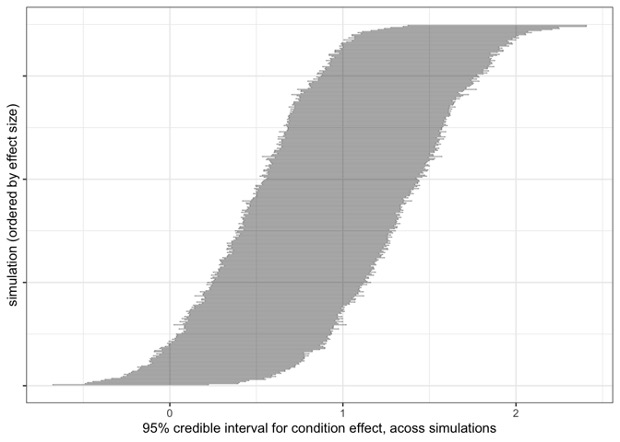
\includegraphics[width=6in]{/Users/mellischreiner/Documents/GitHub/mb2-analysis/paper/Figure3} \hfill{}

\caption{Effect sizes of simulated experiments. \newline{} \textit{Note}. Ordered by effect size (from left to right), 95\% credible intervals for the key effect (in logit space) for our simulated experiments that use first look as the dependent variable.}\label{fig:figS4}
\end{figure}

\subsection{Questionnaires and test session information}\label{questionnaires-and-test-session-information}

Using a questionnaire (filled out during the lab session or online for remote testing procedures) we will collect the following demographic information from the participating toddlers: gender, chronological age in days, nationality of the toddler, estimated proportion of language exposure, preterm/full-term status, current visual or hearing impairments, any known developmental concerns, information about siblings (number, gender, age), duration of time the toddler spends with caregivers and in day-care. From their caregivers the following information will be collected: gender, nationality, native language(s), level of education. For the adult sample, the following demographic information will be collected: gender, chronological age in years, and level of education.
Additionally, we collect the following information for each participant: name of lab the participant was tested in, academic status of the experimenter involved in the test session (e.g., volunteer, undergraduate, graduate, post-doctoral, professor), the type of eye-tracking apparatus used including sampling rate and screen dimensions (for eye-tracking procedures), date of testing, trial order condition the participant was assigned to, any procedural or technical error that occurred during the session and further reasons for exclusion, and the type of recruitment method the lab used. For the toddlers sample, we will additionally ask for the amount of experience the experimenter has in testing toddlers, and whether the toddler sat on the caregiver's lap or in a seat. The requested demographic information that is not used in the registered confirmatory and/or exploratory analyses of this study will be collected for further potential follow-up analyses in spin-off projects within the MB framework.

\subsection{Stimuli}\label{stimuli}

\subsubsection{General Scene Setup}\label{general-scene-setup}

The depicted scene comprises an open space colored in blue. A horizontal picket fence divides the space into two sections (upper: approx. one third; lower: approx. two thirds). In the upper section, initially two animated, same-sized agents are seen: a brown bear (chaser) and a yellow mouse (chasee). The agents communicate using pseudo utterances. When they move, footsteps can be heard. The back of the upper section is formed by a wall with a small, central door through which the agents can enter and leave the scenario. Leaving through this door partially covers the agent, with the lower part of the body still visible. In the lower section of the scene, two identical brown boxes with moveable lids are located (one on the left and one on the right side). A white, centrally located, inverted Y-shaped tunnel connects both sides of the fence. One entrance is located in the upper section, while two identical exits are located in the lower section. Each exit in the lower section points towards the left or right box, respectively. The agents can move from the upper to the lower section of the scene by walking through the tunnel.

\subsubsection{Familiarization Trials}\label{familiarization-trials}

All participants will view four familiarization trials. Each trial starts with the chaser and the chasee playing tag in the upper section of the scene. That is, the chasee runs off in a circle and is closely followed by the chaser (\textasciitilde4 s). When the chasee stops, the chaser catches up and they do a high five (\textasciitilde1 s). After separating again, the agents stand next to each other in front of the tunnel´s entrance (left or right position counterbalanced) (\textasciitilde3 s). Next, the chasee makes eye contact with the chaser (\textasciitilde2 s) and leaves for the tunnel. The chaser watches closely as the chasee walks towards the tunnel and enters it (\textasciitilde2 s). The chaser then positions itself centrally in front of the tunnel entrance (\textasciitilde4 s). While the chasee is walking through the tunnel for four seconds, there is a sound of footsteps. The footsteps cease when the chasee leaves the tunnel through one of the two exits (left or right, counterbalanced) in the lower section (\textasciitilde3 s). At this point, the chasee briefly stops, turns around and establishes eye contact with the chaser across the fence (\textasciitilde1 s). The chaser raises their hands to the mouth and shouts (\textasciitilde2 s). Next, the chasee continues towards the box at the tunnel exit (\textasciitilde1 s). The lid of the box opens (accompanied by a clap sound) and the chasee jumps into it - after which the lid of the box closes, again accompanied by a clap sound (\textasciitilde1 s). Then, the chaser walks towards the tunnel entrance (\textasciitilde2 s) and transits through the tunnel. While it is walking through the tunnel, footsteps sound (\textasciitilde4 s - anticipatory period). After leaving the tunnel (\textasciitilde2 s), the chaser approaches the box in which the chasee is hiding and knocks on it (\textasciitilde2 s). Then, the chasee jumps out of the box (with a box opening clap sound) and the chaser and chasee do a high five (\textasciitilde4 s).

\subsubsection{Test Trials}\label{test-trials}

Test trials start with the same chasing sequence as in the familiarization trials. After doing a high five, chaser and chasee take their positions in front of the tunnel entrance. Next, the chasee makes eye contact with the chaser, leaves for the tunnel and enters it. From this point onwards, the events depend on the condition:
In the ignorance condition, after the chasee entered the tunnel (\textasciitilde12 s after start), the chaser exits through the door in the wall in the back (\textasciitilde4 s). The back of the chaser remains visible. While the chaser is away (for \textasciitilde8 s), the chasee walks through the tunnel (\textasciitilde4 s) and leaves through one of the exits (left or right, counterbalanced)(\textasciitilde2 s) and jumps into the respective box (\textasciitilde1 s). After approximately one second, while the chaser is still away, the chasee leaves this box A and tiptoes to the other box (\textasciitilde4 s). The chasee then jumps into box B and the lid closes (\textasciitilde1 s). In contrast to the familiarization trials, the chasee and the boxes make no sounds and no chime is played. After the hiding event has finished, the chaser returns through the door in the wall (\textasciitilde3 s) and enters the tunnel (\textasciitilde2 s). While the chaser is in the tunnel, footsteps are heard (\textasciitilde4 s). The video ends before the chaser exits the tunnel.
In the knowledge condition, the chaser remains on the scene in the upper section and positions itself centrally in front of the tunnel entrance (\textasciitilde2 s). Following the same sequence as in the ignorance condition, the chasee walks through the tunnel (\textasciitilde2 s), leaves it through one of the exits (left or right, counterbalanced) (\textasciitilde2 s) and hides in the respective box (\textasciitilde1 s). Next, in order to match the events of the ignorance condition, the chaser walks towards the door in the wall (\textasciitilde3 s) and disappears for approximately 1 seconds. Subsequently, they return to the initial position in front of the tunnel entrance (\textasciitilde3 s). In the meantime, the chasee did not move, so that the chaser did not miss any events while they were gone. Once the chaser returns it observes the chasee jump out of the first box (\textasciitilde1 s) and tiptoe to the second box (\textasciitilde4 s). Finally, the chasee jumps into the second box and the lid closes (\textasciitilde1 s). Like in the ignorance condition, the chasee and the boxes make no sound and no chime is played. The chaser enters the tunnel (\textasciitilde2 s) and footsteps sound (\textasciitilde4 s). Like in the ignorance condition, the video ends before the chaser exits the tunnel.

\subsubsection{Trial randomization}\label{trial-randomization}

The four combinations in familiarization were the following: started from the right and ended up in right box (RR); started from the right and ended up in left box (RL); started from the left and ended up in right box (LR); started from the left and ended up in left box (LL). The presentation of the familiarization trials will be counterbalanced in two pseudo-randomized orders (familiarization order A: Fam\_LR, Fam\_LL, Fam\_RL, Fam\_RR; familiarization order B: Fam\_RL, Fam\_RR, Fam\_LR, Fam\_LL). As with the familiarization trials, there will be four different parallel versions of the test trial for the knowledge and the ignorance condition, differing in the starting location of the chasee and the box the chasee ended up (Know\_RR, Know\_RL, Know\_LR, Know\_LL; Ig\_RR, Ig\_RL, Ig\_LR, Ig\_LL). Supplementary Table S2 lists the combinations that will be tested. Each lab signs up for one or two trial bins (16 trial combinations per bin) for each tested age group.

\subsection{General Lab Practices}\label{general-lab-practices}

\subsubsection{Training of Research Assistants}\label{training-of-research-assistants}

Each participating lab is responsible for maintaining the highest possible experimental standards, providing training practices for all experimenters and research assistants, and following detailed, written instructions to achieve uniformity and minimize variation across labs. Individual labs will document which experimenter(s) and research assistant(s) will test each participant. A questionnaire will serve to record and compare training practices. Greeting practices and instructions given to the participant/caregiver are marked down and standardized.

\subsubsection{Reporting of Technology Mishaps and Participant/Caregiver Behavior}\label{reporting-of-technology-mishaps-and-participantcaregiver-behavior}

All labs are required to report anomalies, technical issues, concerns, and general comments on the protocol sheet. For toddler samples, concerns and general comments comprise the following: crying, fussiness, weariness, caregiver intervening (verbal or non-verbal, e.g., pointing), affecting or disrupting participation and/or looking behavior. Technical issues include problems that hinder, pause, or stop the stimulus presentation and/or eye-tracking recording.

\subsection{Participant exclusion}\label{participant-exclusion}

Of the initial sample (toddlers: \emph{N} = 809, adults: \emph{N} = 805), participants will be excluded from the main confirmatory analyses if:
They did not complete the full experiment (toddlers: \emph{n} = 26, 3.21\%; adults: \emph{n} = 0, 0\%),
Participants' caregivers interfered with the procedure, e.g., by pointing at stimuli or talking to their toddler (toddlers: \emph{n} = 11, 1.36\%; adults: \emph{n} = 0, 0\%),
the experimenter made an error during testing that was relevant to the procedure (toddlers: \emph{n} = 11, 1.36\%; adults: \emph{n} = 6, 0.75\%),
technical problems occurred, e.g., data not saved, unable to calibrate eye-tracker, eye-tracker lost signal, data loss due to computer failure, computer crashed during recording (toddlers: \emph{n} = 69, 8.53\%; adults: \emph{n} = 61, 7.58\%).
The individual labs will determine whether and to which extent participant exclusion criteria 1-4 apply and add this information to the participant protocol sheet they provide. This set of exclusions will leave a total of 703 toddlers and 736 adults whose data will be analyzed. Of these, participants will be excluded sequentially if:
5. Their data were excluded due to missingness (see Preprocessing section) from more than one familiarization trial (toddlers: \emph{n} = 112, 13.84\%; adults: \emph{n} = 24, 2.98\%),
6. Their data from the first (critical) test trial were excluded due to missingness (toddlers: \emph{n} = 54, 6.67\%; adults: \emph{n} = 9, 1.12\%).
If multiple reasons for exclusion are applicable to a participant, the criteria will be assigned in the order above.

\section{S3. Further Supplemental Information: Analysis}\label{s3.-further-supplemental-information-analysis}

\subsection{Secondary analysis with less informative prior}\label{secondary-analysis-with-less-informative-prior}

To evaluate the sensitivity of our findings to prior assumptions, we performed two Bayesian analyses for each phase (familiarization and test) and age cohort (toddlers and adults). The first analysis used weakly informative priors, reflecting modest assumptions about effect sizes and variability (as presented in the main manuscript). The second analysis employed less-informative priors, allowing for greater flexibility in parameter estimation. In particular, fixed effect coefficients were modeled with a normal prior (N(0,3)), and random effect standard deviations were modeled with a normal prior (N(0,0.5)). See Table S3 for a summary of the results using both priors across age cohorts and phases.

In the familiarization phase, the results were consistent and robust across both toddlers and adults, regardless of the prior specification. Parameter estimates, such as the effect of trial number, indicated clear evidence of learning or habituation. Bayes Factors strongly favored the models over the null hypothesis, reflecting high confidence in the observed effects. This consistency across weakly informative and less informative priors underscores the reliability of the findings in this phase, suggesting that the observed patterns are driven by the data rather than being influenced by prior assumptions.

The test phase for toddlers showed greater sensitivity to prior specifications. While parameter estimates remained relatively stable, the Bayes Factor results were much more variable, especially when evidence for the model was marginal. Under the weakly informative prior, the
Bayes Factor suggested modest support for the model; however, the less informative prior yielded an almost negligible Bayes Factor, indicating little evidence favoring the model over the null. These differences highlight the importance of careful interpretation of results in contexts where the data provide only weak evidence, as conclusions in such cases are more influenced by prior assumptions.

In the test phase for adults, the results also displayed some sensitivity to prior specification, though to a lesser extent than in the toddler group. Parameter estimates remained consistent, with clear evidence for an effect of condition. The Bayes Factor, while robust across priors, was lower under the less informative prior compared to the weakly informative one. This indicates that although the adult test phase results are reliable, the strength of evidence can be moderated by the choice of priors, especially when comparing models with relatively flexible assumptions.

The analyses demonstrate that parameter estimates were generally robust across prior specifications, highlighting the stability of the data-driven conclusions. However, Bayes Factors were notably more sensitive to prior choices, particularly in cases where the evidence for the model was less compelling, such as in the toddlers' test phase. In the familiarization phase, results were strong for both toddlers and adults, regardless of prior specification. In contrast, prior sensitivity was greater in the test phase, especially for toddlers, where evidence for the model was weaker. These findings underscore the importance of reporting analyses with multiple priors to enhance transparency and robustness. They also caution against overinterpreting Bayes Factors in cases where priors are highly flexible or the evidence is marginal.

\begin{table}
\centering
\caption{\label{tab:unnamed-chunk-2}Summary of Bayesian Results Across Phases and Priors.}
\centering
\resizebox{\ifdim\width>\linewidth\linewidth\else\width\fi}{!}{
\begin{threeparttable}
\begin{tabular}[t]{lllrll}
\toprule
Age Cohort & Phase & Prior & Bayes Factor & Parameter Estimates & Sensitivity\\
\midrule
Toddlers & Familiarization & Weakly Informative & 7180 & Intercept: 0.44, Main Effect: -0.22 & Low\\
 &  & Less Informative & 10763 & Intercept: 0.45, Main Effect: -0.23 & Low\\
Adults &  & Weakly Informative & 2242713044 & Intercept: 1.03, Main Effect: 0.38 & Low\\
 &  & Less Informative & 5201436143831125852160 & Intercept: 1.06, Main Effect: 0.40 & Low\\
Toddlers & Test & Weakly Informative & 2.4 & Intercept: 0.53, Main Effect: 0.53, Interaction: -0.13 & High\\
\addlinespace
 &  & Less Informative & 1 & Intercept: 0.57, Main Effect: 0.56, Interaction: -0.14 & High\\
Adults &  & Weakly Informative & 157455 & Intercept: 0.05, Main Effect: -0.89 & Moderate\\
 &  & Less Informative & 1889 & Intercept: 0.06, Main Effect: -0.96 & Moderate\\
\bottomrule
\end{tabular}
\begin{tablenotes}[para]
\item \textit{Note: } 
\item BFs reported for the familiarization phase are model comparisons without the intercept. BFS reported for the test phase are model comparisons without the fixed effect of condition.
\end{tablenotes}
\end{threeparttable}}
\end{table}

\subsection{Data collection type: in-lab vs.~web-based}\label{data-collection-type-in-lab-vs.-web-based}

In analyses introducing model terms for certain measurement characteristics (e.g., types of eye-tracker manufacturers, screen dimensions), we will quantify potential variability between different in-lab data acquisition methods (cf., ManyBabies Consortium, 2020). If we have a sufficiently large sample of participants tested with online sources (e.g., contributions of at least 32 participants), we will conduct a separate analysis with a model term for online participants that estimates whether condition effects are different in this population. We will further report whether exclusion rates are different for this population.

Bayesian mixed-effects models were used to evaluate the effects of condition, method, and their interaction on anticipatory looking. The models included fixed effects for condition, method, and their interaction. For toddlers, the effect of method was small and uncertain, with the credible interval including zero, indicating no clear effect of method. The interaction between condition and method was minimal and also uncertain, suggesting no strong evidence that the effect of condition varied by method. The estimated Bayes factor comparing the full model to the null model was approximately BF = 0.7, which indicates that the data slightly favors the null model over the full model. This suggests that the predictors included in the full model do not substantially improve the explanation of the observed data compared to the null model.

For adults, the main effect of method was slightly negative but uncertain, suggesting that the method had little to no clear effect on the outcome. The interaction between condition and method was negative but with a wide credible interval crossing zero, indicating uncertainty about whether the effect of condition varied by method. The estimated Bayes factor in favor of the full model over the null model was BF = 2.9. This Bayes factor indicates that the evidence in favor of the model is modest but not strong. While the model is more likely than the null model to explain the observed data, the support is relatively weak, suggesting that the predictors in the model provide only a small improvement in explaining the data compared to the null model.

In sum, the analysis suggests that the method used (web-based vs.~in-lab) does not have a strong impact on AL, as the effect of method and its interaction with condition were small and uncertain. Additionally, the results should be interpreted with caution due to the relatively small sample size for web-based data compared to in-lab data collection, which may limit the robustness of the findings.

\subsection{AL as a function of differential fixation times of bear and mouse during location change of the mouse}\label{al-as-a-function-of-differential-fixation-times-of-bear-and-mouse-during-location-change-of-the-mouse}

In order to examine the effect of condition and the difference in looking times for mouse and bear during location change of the mouse on anticipatory looking, we fitted a Bayesian mixed-effects model for both age cohorts separately. The dependent variable was the proportion DLS. The fixed effects included the main effects of condition, the difference in fixation times of mouse and bear, and their interaction. We also included random intercepts and slopes for differences in fixation times of mouse and bear within each participant and within each lab, allowing us to account for the hierarchical structure of the data and potential variability between labs and participants.

Due to limitations with bridge sampling, Bayes factors were computed using the Savage-Dickey density ratio method. These analyses provided moderate evidence against including both the fixed effect of difference in fixation times of mouse and bear, BF = 0.3, and its interaction with condition, BF = 0.2. These results suggest that the difference in looking time to mouse versus bear, either alone or in interaction with condition, did not meaningfully account for variance in toddlers' proportional DLS.

To assess whether proportional DLS in adults was predicted by condition, the difference in looking time between the mouse and bear, and their interaction, we fit a Bayesian mixed-effects model. There was a strong negative main effect of condition, indicating lower proportional DLS in the ignorance condition compared to the knowledge condition (Estimate = --0.21, 95\% CI {[}--0.29, --0.13{]}). We also observed a negative main effect of mouse-bear looking difference, with greater looking toward the bear (relative to the mouse) associated with higher proportion DLS (Estimate = --0.04, 95\% CI {[}--0.05, --0.02{]}). The interaction between condition and looking difference was close to zero and uncertain (Estimate = 0.01, 95\% CI {[}--0.02, 0.04{]}).

Bayes factors computed using the Savage-Dickey method provided overwhelming evidence in favor of including the fixed effect of the difference in looking time between the mouse and bear, BF \textgreater{} 1000, and moderate evidence against including the interaction term, BF = 0.2. These results suggest that both condition and mouse-versus-bear looking independently predict proportional DLS in adults, but their interaction does not appear to contribute meaningfully.

\begin{figure}

{\centering 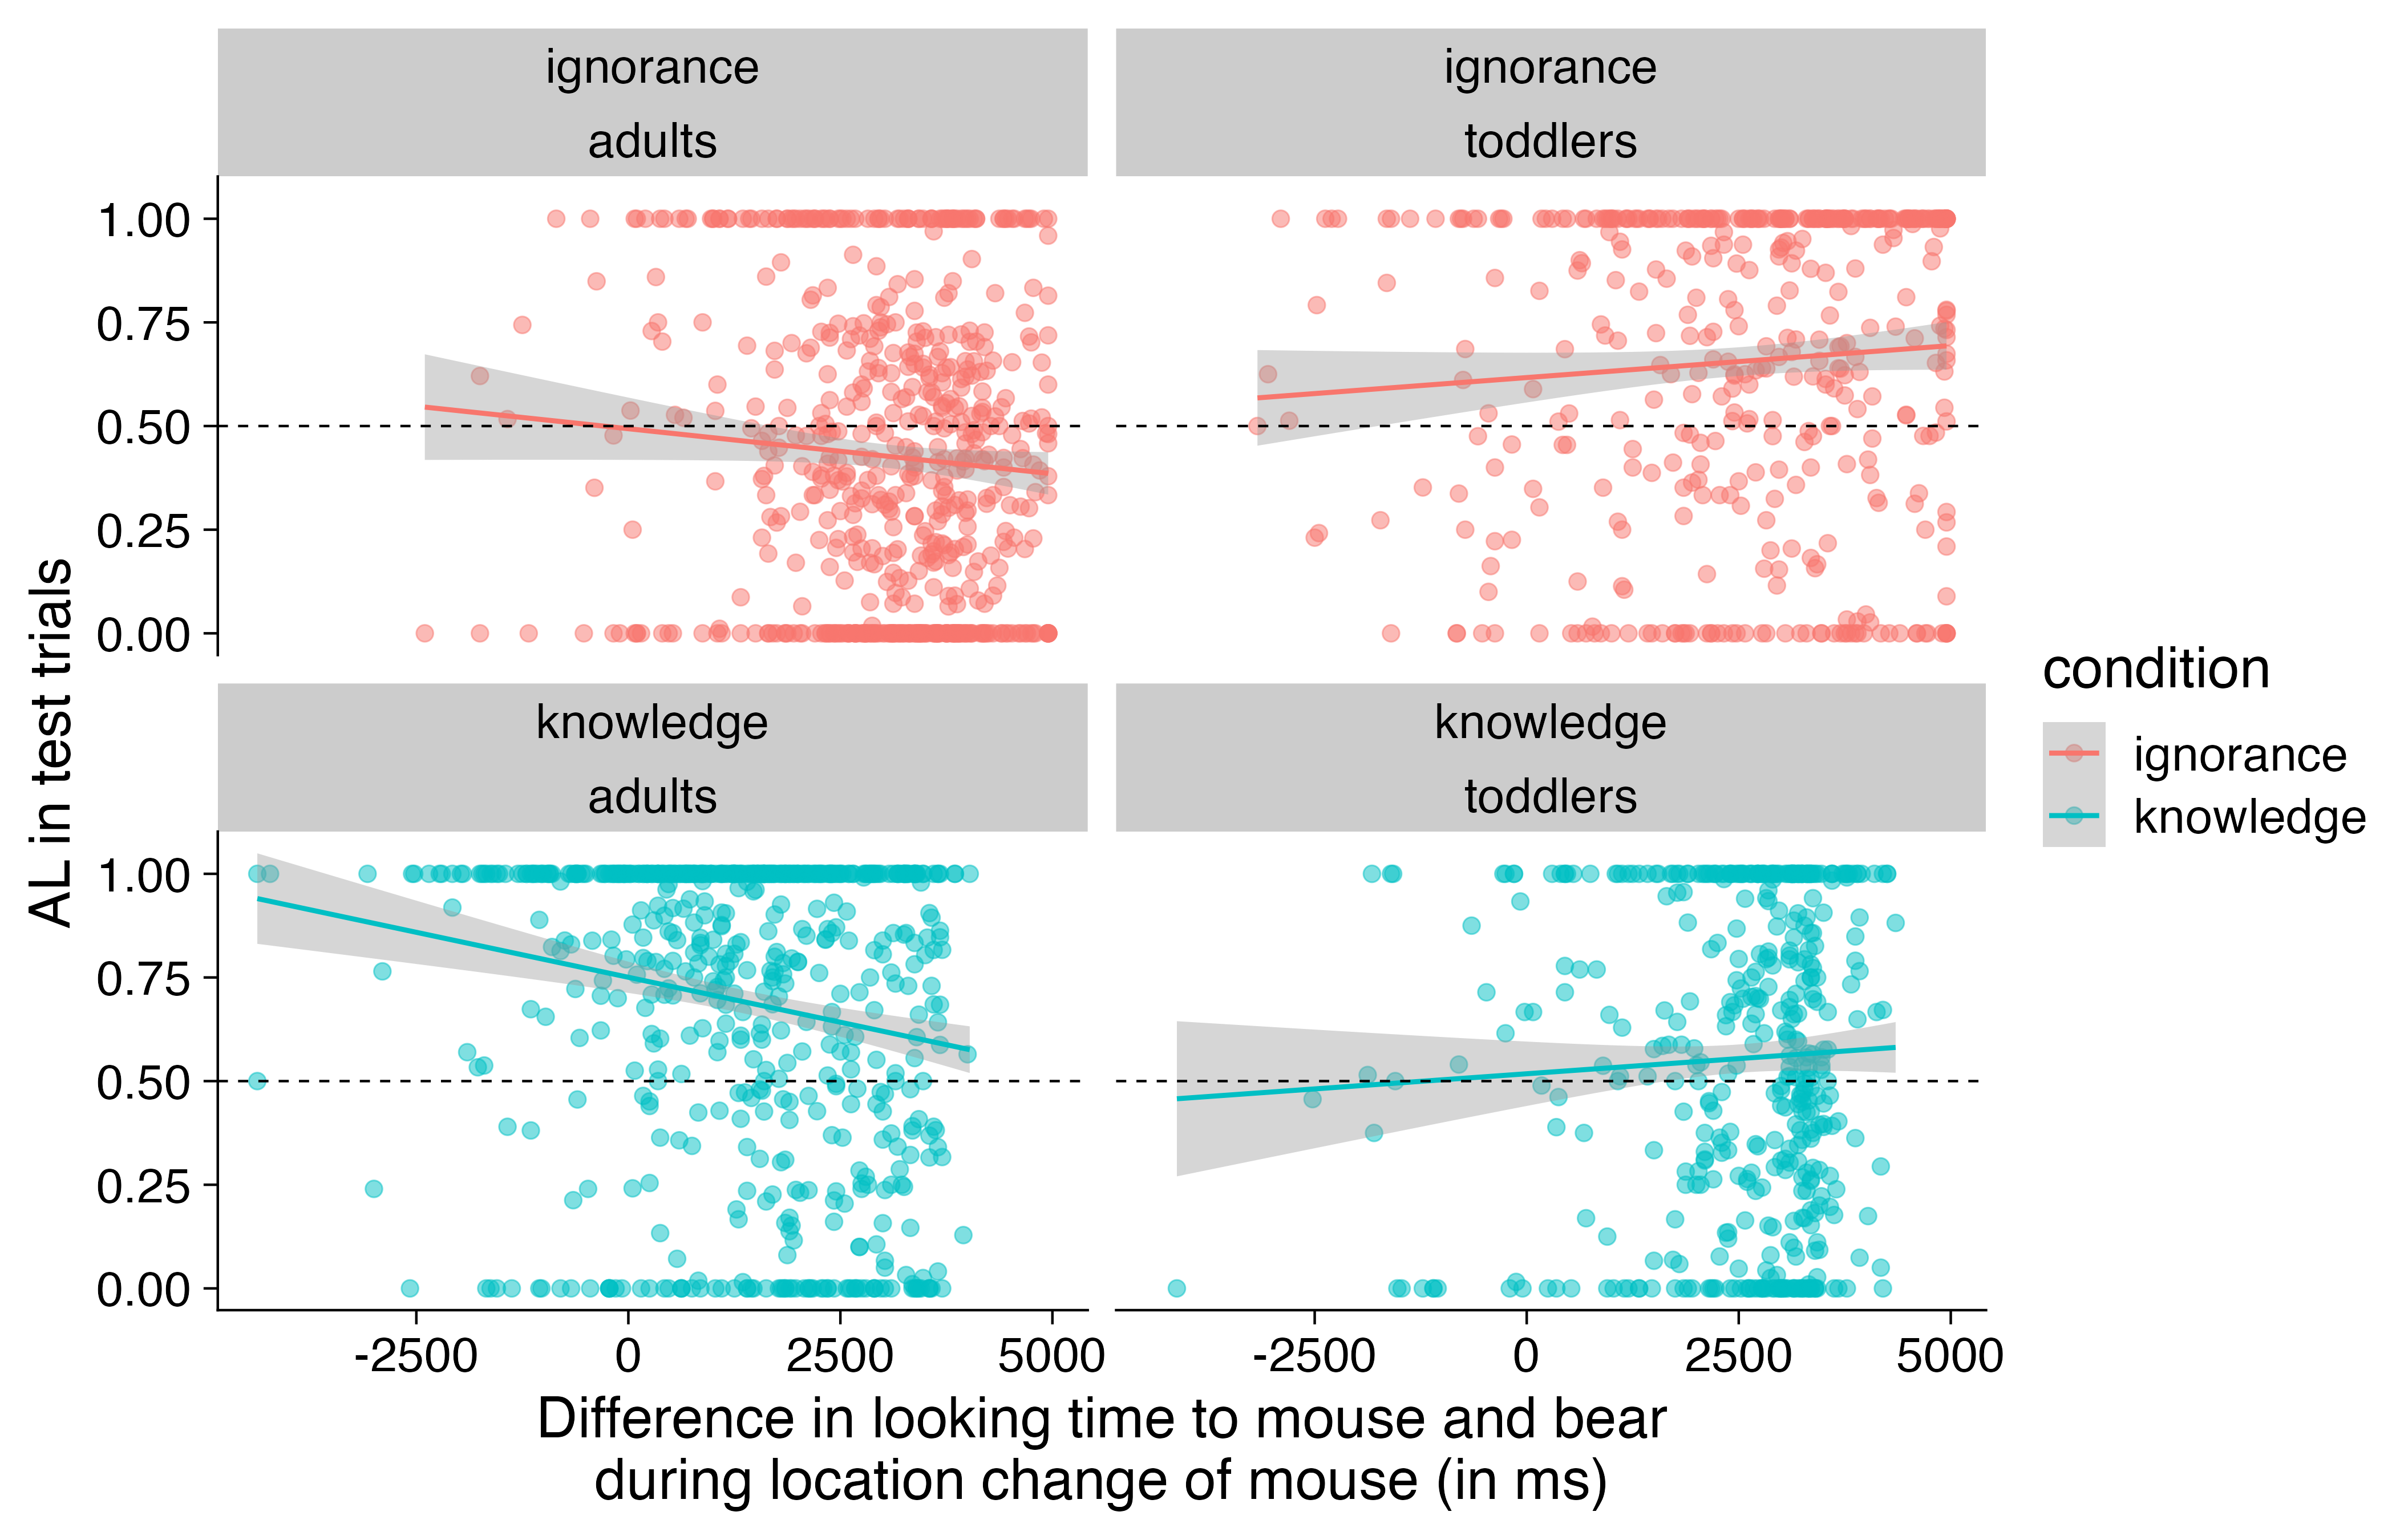
\includegraphics[width=6.8in]{/Users/mellischreiner/Documents/GitHub/mb2-analysis/paper/Figure8} 

}

\caption{AL as a function of the difference in looking time to mouse and bear during location change of mouse (in ms) for each age cohort and each condition.}\label{fig:fig10}
\end{figure}

\subsection{Influence of target location from previous trials}\label{influence-of-target-location-from-previous-trials}

\subsubsection{Test phase: Influence of target location from last familarization on proportional target looking in first test trial}\label{test-phase-influence-of-target-location-from-last-familarization-on-proportional-target-looking-in-first-test-trial}

We examined whether proportion DLS in the first test trial was influenced by condition, the location of the target in the preceding familiarization trial (same vs.~different), and their interaction. Separate Bayesian mixed-effects models were fitted for toddlers and adults, including random intercepts and slopes for condition by lab.

For toddlers, we found a significant effect of condition, with higher proportion DLS in the ignorance condition compared to the knowledge condition. The effect of location and the interaction between condition and location were not significant (see Table S3). A model comparison testing the inclusion of the location effect yielded a Bayes factor of BF = 0.9, indicating anecdotal evidence against its contribution. A Bayes factor comparison indicated anecdotal evidence against the interaction model, with
BF = 0.6.

For adults, results similarly revealed a significant effect of condition, with greater proportion DLS in the knowledge condition. The main effect of location and the interaction were not significant. The model comparison testing the main effect of location yielded a Bayes factor of BF = 0.3, suggesting moderate evidence against its inclusion. A Bayes factor comparison suggested anecdotal evidence against the inclusion of the interaction term, with BF = 0.8.

\subsubsection{Familiarization phase: Influence of target location from previous familiarization trials on proportional target looking}\label{familiarization-phase-influence-of-target-location-from-previous-familiarization-trials-on-proportional-target-looking}

We also assessed whether proportion DLS during the familiarization phase was influenced by the target's location in the previous trial, trial number, and their interaction. Separate Bayesian mixed-effects models were fitted for toddlers and adults, with random intercepts for participants and labs.

For toddlers, there was a significant negative effect of previous trial location (see Table S3), indicating that toddlers looked more at the target when it had been on the same side as in the previous trial. The effect of trial number and the interaction were not significant. The model comparison testing the contribution of the location effect alone yielded a Bayes Factor of BF \textgreater{} 1000, indicating extreme evidence in favor of including previous trial location. Furthermore, a Bayes factor analysis provided anecdotal evidence in favor of the full model compared to the null model without the interaction of these predictors, BF = 1.1.

For adults, no predictor reached significance. The Bayes factor for including location was BF = 1.3, providing only anecdotal support for its contribution. The Bayes factor, BF = 0.4, further supports the conclusion that the model including the interaction of the predictors was not substantially better than the null model, providing anecdotal evidence for the null model.

\begin{figure}

{\centering 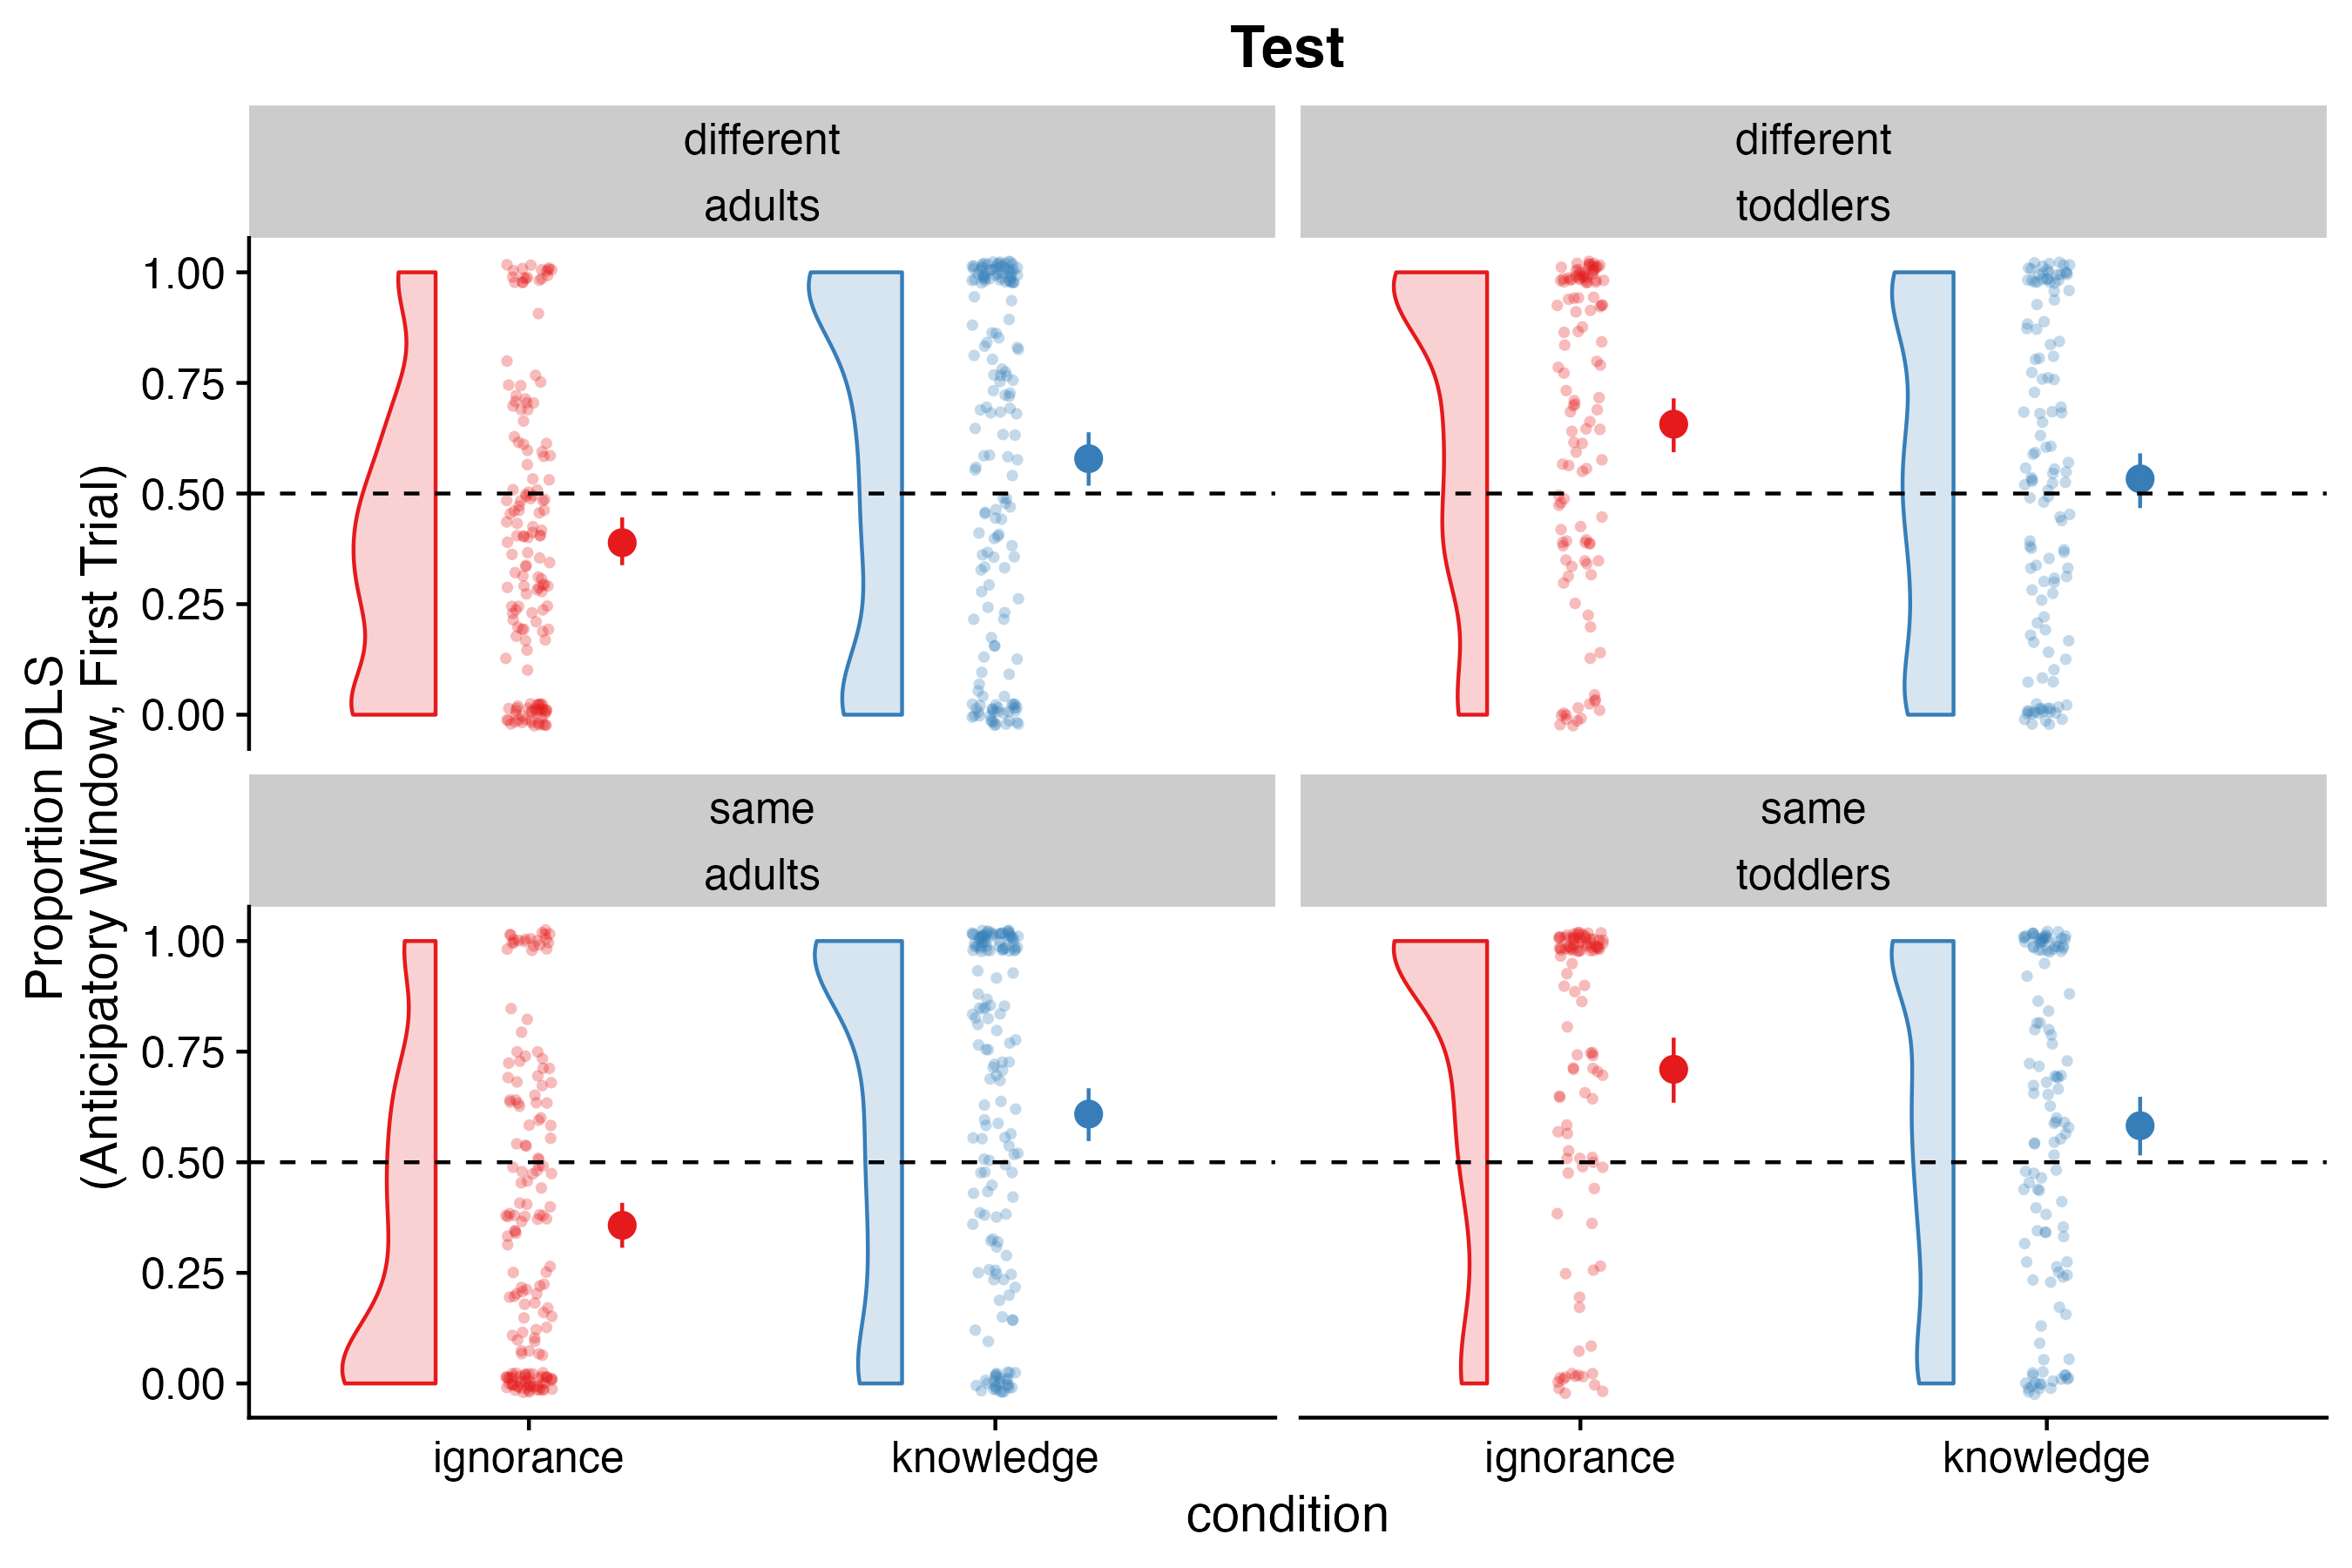
\includegraphics[width=6.8in]{/Users/mellischreiner/Documents/GitHub/mb2-analysis/paper/FigureS6} 

}

\caption{Proportion DLS during the first test trial for toddlers and adults split by condition (knowledge vs. ignorance) and consistency of location in the previous familiarization trial (same vs. different). Error bars represent 95\% CIs.}\label{fig:fig11}
\end{figure}

\begin{center}
\begin{ThreePartTable}

\footnotesize{

\begin{longtable}{llrrrrr}\noalign{\getlongtablewidth\global\LTcapwidth=\longtablewidth}
\caption{\label{tab:Results table of Bayesian mixed effects models proportional target looking was influenced by the location of the target in the previous trial}Results of the Bayesian mixed effects models for consitency of location.}\\
\toprule
model & \multicolumn{1}{c}{term} & \multicolumn{1}{c}{estimate} & \multicolumn{1}{c}{est\_error} & \multicolumn{1}{c}{lower\_ci} & \multicolumn{1}{c}{upper\_ci} & \multicolumn{1}{c}{rhat}\\
\midrule
\endfirsthead
\caption*{\normalfont{Table \ref{tab:Results table of Bayesian mixed effects models proportional target looking was influenced by the location of the target in the previous trial} continued}}\\
\toprule
model & \multicolumn{1}{c}{term} & \multicolumn{1}{c}{estimate} & \multicolumn{1}{c}{est\_error} & \multicolumn{1}{c}{lower\_ci} & \multicolumn{1}{c}{upper\_ci} & \multicolumn{1}{c}{rhat}\\
\midrule
\endhead
test adults & Intercept & 0.48 & 0.02 & 0.45 & 0.52 & 1.00\\
 & Condition & -0.20 & 0.03 & -0.26 & -0.15 & 1.00\\
 & Location & 0.00 & 0.03 & -0.05 & 0.05 & 1.00\\
 & Condition:Location & 0.05 & 0.05 & -0.05 & 0.14 & 1.00\\
test toddlers & Intercept & 0.62 & 0.02 & 0.59 & 0.66 & 1.00\\
 & Condition & 0.11 & 0.03 & 0.05 & 0.18 & 1.00\\
 & Location & -0.04 & 0.03 & -0.11 & 0.02 & 1.00\\
 & Condition:Location & 0.00 & 0.06 & -0.11 & 0.11 & 1.00\\
fam adults & Intercept & 0.18 & 0.02 & 0.14 & 0.23 & 1.00\\
 & Location & 0.06 & 0.04 & -0.02 & 0.14 & 1.00\\
 & Trial Number & -0.02 & 0.04 & -0.09 & 0.05 & 1.00\\
 & Location:Trial Number & 0.07 & 0.07 & -0.07 & 0.21 & 1.00\\
fam toddlers & Intercept & 0.17 & 0.02 & 0.13 & 0.21 & 1.00\\
 & Location & -0.17 & 0.03 & -0.23 & -0.10 & 1.00\\
 & Trial Number & 0.01 & 0.03 & -0.05 & 0.08 & 1.00\\
 & Location:Trial Number & -0.01 & 0.06 & -0.14 & 0.11 & 1.00\\
\bottomrule
\end{longtable}

}

\end{ThreePartTable}
\end{center}

\newpage

\section{References}\label{references}

\begingroup
\setlength{\parindent}{-0.5in}
\setlength{\leftskip}{0.5in}

\phantomsection\label{refs}
\begin{CSLReferences}{1}{0}
\bibitem[\citeproctext]{ref-kampis2020altercentric}
Kampis, D., \& Southgate, V. (2020). Altercentric cognition: How others influence our cognitive processing. \emph{Trends in Cognitive Sciences}, \emph{24}(11), 945--959.

\bibitem[\citeproctext]{ref-manybabies2020quantifying}
ManyBabies Consortium. (2020). Quantifying sources of variability in infancy research using the infant-directed-speech preference. \emph{Advances in Methods and Practices in Psychological Science}, \emph{3}(1), 24--52.

\bibitem[\citeproctext]{ref-schuwerk2018robustness}
Schuwerk, T., Priewasser, B., Sodian, B., \& Perner, J. (2018). The robustness and generalizability of findings on spontaneous false belief sensitivity: A replication attempt. \emph{Royal Society Open Science}, \emph{5}(5), 172273.

\bibitem[\citeproctext]{ref-southgate2007action}
Southgate, V., Senju, A., \& Csibra, G. (2007). Action anticipation through attribution of false belief by 2-year-olds. \emph{Psychological Science}, \emph{18}(7), 587--592.

\end{CSLReferences}

\endgroup


\end{document}
